% Options for packages loaded elsewhere
\PassOptionsToPackage{unicode}{hyperref}
\PassOptionsToPackage{hyphens}{url}
%
\documentclass[
  12pt,
]{article}
\usepackage{amsmath,amssymb}
\usepackage{lmodern}
\usepackage{iftex}
\ifPDFTeX
  \usepackage[T1]{fontenc}
  \usepackage[utf8]{inputenc}
  \usepackage{textcomp} % provide euro and other symbols
\else % if luatex or xetex
  \usepackage{unicode-math}
  \defaultfontfeatures{Scale=MatchLowercase}
  \defaultfontfeatures[\rmfamily]{Ligatures=TeX,Scale=1}
  \setmainfont[]{Times New Roman}
\fi
% Use upquote if available, for straight quotes in verbatim environments
\IfFileExists{upquote.sty}{\usepackage{upquote}}{}
\IfFileExists{microtype.sty}{% use microtype if available
  \usepackage[]{microtype}
  \UseMicrotypeSet[protrusion]{basicmath} % disable protrusion for tt fonts
}{}
\makeatletter
\@ifundefined{KOMAClassName}{% if non-KOMA class
  \IfFileExists{parskip.sty}{%
    \usepackage{parskip}
  }{% else
    \setlength{\parindent}{0pt}
    \setlength{\parskip}{6pt plus 2pt minus 1pt}}
}{% if KOMA class
  \KOMAoptions{parskip=half}}
\makeatother
\usepackage{xcolor}
\usepackage[margin=2.54cm]{geometry}
\usepackage{color}
\usepackage{fancyvrb}
\newcommand{\VerbBar}{|}
\newcommand{\VERB}{\Verb[commandchars=\\\{\}]}
\DefineVerbatimEnvironment{Highlighting}{Verbatim}{commandchars=\\\{\}}
% Add ',fontsize=\small' for more characters per line
\usepackage{framed}
\definecolor{shadecolor}{RGB}{248,248,248}
\newenvironment{Shaded}{\begin{snugshade}}{\end{snugshade}}
\newcommand{\AlertTok}[1]{\textcolor[rgb]{0.94,0.16,0.16}{#1}}
\newcommand{\AnnotationTok}[1]{\textcolor[rgb]{0.56,0.35,0.01}{\textbf{\textit{#1}}}}
\newcommand{\AttributeTok}[1]{\textcolor[rgb]{0.77,0.63,0.00}{#1}}
\newcommand{\BaseNTok}[1]{\textcolor[rgb]{0.00,0.00,0.81}{#1}}
\newcommand{\BuiltInTok}[1]{#1}
\newcommand{\CharTok}[1]{\textcolor[rgb]{0.31,0.60,0.02}{#1}}
\newcommand{\CommentTok}[1]{\textcolor[rgb]{0.56,0.35,0.01}{\textit{#1}}}
\newcommand{\CommentVarTok}[1]{\textcolor[rgb]{0.56,0.35,0.01}{\textbf{\textit{#1}}}}
\newcommand{\ConstantTok}[1]{\textcolor[rgb]{0.00,0.00,0.00}{#1}}
\newcommand{\ControlFlowTok}[1]{\textcolor[rgb]{0.13,0.29,0.53}{\textbf{#1}}}
\newcommand{\DataTypeTok}[1]{\textcolor[rgb]{0.13,0.29,0.53}{#1}}
\newcommand{\DecValTok}[1]{\textcolor[rgb]{0.00,0.00,0.81}{#1}}
\newcommand{\DocumentationTok}[1]{\textcolor[rgb]{0.56,0.35,0.01}{\textbf{\textit{#1}}}}
\newcommand{\ErrorTok}[1]{\textcolor[rgb]{0.64,0.00,0.00}{\textbf{#1}}}
\newcommand{\ExtensionTok}[1]{#1}
\newcommand{\FloatTok}[1]{\textcolor[rgb]{0.00,0.00,0.81}{#1}}
\newcommand{\FunctionTok}[1]{\textcolor[rgb]{0.00,0.00,0.00}{#1}}
\newcommand{\ImportTok}[1]{#1}
\newcommand{\InformationTok}[1]{\textcolor[rgb]{0.56,0.35,0.01}{\textbf{\textit{#1}}}}
\newcommand{\KeywordTok}[1]{\textcolor[rgb]{0.13,0.29,0.53}{\textbf{#1}}}
\newcommand{\NormalTok}[1]{#1}
\newcommand{\OperatorTok}[1]{\textcolor[rgb]{0.81,0.36,0.00}{\textbf{#1}}}
\newcommand{\OtherTok}[1]{\textcolor[rgb]{0.56,0.35,0.01}{#1}}
\newcommand{\PreprocessorTok}[1]{\textcolor[rgb]{0.56,0.35,0.01}{\textit{#1}}}
\newcommand{\RegionMarkerTok}[1]{#1}
\newcommand{\SpecialCharTok}[1]{\textcolor[rgb]{0.00,0.00,0.00}{#1}}
\newcommand{\SpecialStringTok}[1]{\textcolor[rgb]{0.31,0.60,0.02}{#1}}
\newcommand{\StringTok}[1]{\textcolor[rgb]{0.31,0.60,0.02}{#1}}
\newcommand{\VariableTok}[1]{\textcolor[rgb]{0.00,0.00,0.00}{#1}}
\newcommand{\VerbatimStringTok}[1]{\textcolor[rgb]{0.31,0.60,0.02}{#1}}
\newcommand{\WarningTok}[1]{\textcolor[rgb]{0.56,0.35,0.01}{\textbf{\textit{#1}}}}
\usepackage{longtable,booktabs,array}
\usepackage{calc} % for calculating minipage widths
% Correct order of tables after \paragraph or \subparagraph
\usepackage{etoolbox}
\makeatletter
\patchcmd\longtable{\par}{\if@noskipsec\mbox{}\fi\par}{}{}
\makeatother
% Allow footnotes in longtable head/foot
\IfFileExists{footnotehyper.sty}{\usepackage{footnotehyper}}{\usepackage{footnote}}
\makesavenoteenv{longtable}
\usepackage{graphicx}
\makeatletter
\def\maxwidth{\ifdim\Gin@nat@width>\linewidth\linewidth\else\Gin@nat@width\fi}
\def\maxheight{\ifdim\Gin@nat@height>\textheight\textheight\else\Gin@nat@height\fi}
\makeatother
% Scale images if necessary, so that they will not overflow the page
% margins by default, and it is still possible to overwrite the defaults
% using explicit options in \includegraphics[width, height, ...]{}
\setkeys{Gin}{width=\maxwidth,height=\maxheight,keepaspectratio}
% Set default figure placement to htbp
\makeatletter
\def\fps@figure{htbp}
\makeatother
\setlength{\emergencystretch}{3em} % prevent overfull lines
\providecommand{\tightlist}{%
  \setlength{\itemsep}{0pt}\setlength{\parskip}{0pt}}
\setcounter{secnumdepth}{5}
\ifLuaTeX
  \usepackage{selnolig}  % disable illegal ligatures
\fi
\IfFileExists{bookmark.sty}{\usepackage{bookmark}}{\usepackage{hyperref}}
\IfFileExists{xurl.sty}{\usepackage{xurl}}{} % add URL line breaks if available
\urlstyle{same} % disable monospaced font for URLs
\hypersetup{
  pdftitle={Exploration of 2016-2017 CITES Poaching Database},
  pdfauthor={Emily Wood},
  hidelinks,
  pdfcreator={LaTeX via pandoc}}

\title{Exploration of 2016-2017 CITES Poaching Database}
\usepackage{etoolbox}
\makeatletter
\providecommand{\subtitle}[1]{% add subtitle to \maketitle
  \apptocmd{\@title}{\par {\large #1 \par}}{}{}
}
\makeatother
\subtitle{\url{https://github.com/emilyrwood/CITES_Poaching_Wood}}
\author{Emily Wood}
\date{}

\begin{document}
\maketitle

\newpage
\tableofcontents 
\newpage
\listoftables

Table 1. Processed Data Frame

Table 2. Two Way ANOVA Summary

Table 3. Two Way LM Summary 2

Table 4. Two Way ANOVA comparing dependent variables

Table 5. Model 2 - Two Way ANOVA Summary

Table 6. Model 2 - Two Way LM Summary 2

Table 7. Model 2 - Two Way ANOVA Comparing Class and Appendix

\newpage
\listoffigures

Figure 1. Export Distribution

Figure 2. Import Distribution

Figure 3. Export and Import Quantity

Figure 4. Export and Import Quantity for Appendix I

Figure 5. Importer World Map (In separate Document)

Figure 6. Importer Country Plot Top 10

Figure 7. Exporter World Map (In separate Document)

Figure 8. Exporter Country Plot Top 10

Figure 9. Classes of Poaching Occurrences 2016

Figure 10. Classes of Poaching Occurrences per Appendix Level

Figure 11. Mammalia Class Good Type

Figure 12. Aves Class Good Type

Figure 13. Reptilia Class Good Type

Figure 14. NA Class Good Type

Figure 15. Appendix and Class Compared to Reported Quantity \newpage

\hypertarget{rationale-and-research-questions}{%
\section{Rationale and Research
Questions}\label{rationale-and-research-questions}}

Poaching remains a considerable threat to biodiversity across the
planet. However, it often is overshadowed by other environmental issues
in the policy realm. This is especially true for species that aren't
charismatic mega-fauna. I'm undertaking this research project to better
understand the trends in poaching over time and understand the regions
where the most risk is occuring. This could help target poaching
hotspots and help policy makers make more informed decisions when it
comes to mitigating poaching risk for sesitive species.

\textbf{Main Questions:}

Is there any correlation between class, term, appendix number and
poaching amount?

\textbf{Sub Questions:}

What is the distribution of amounts found exported and imported for all
species included in the database?

Are there differences between Appendix Levels for the amount exported
vs.~imported?

What are the most commonly poached classes between Appendix Levels?

What are the top 3 Classes for species poached in Appendix I?

What are the dominant good types (terms) for the top 3 classes poached
in Appendix I?

Which Counties are the biggest Importer and Exporters of CITES species?

\newpage

\hypertarget{dataset-information}{%
\section{Dataset Information}\label{dataset-information}}

The Convention on International Trade in Endangered Species of Wild
Fauna and Flora (CITES) is an international agreement between
governments. This group studies poaching trends and advises the UN on
necessary action to mitigate this risk. This CITES dataset contains
records on every international import or export conducted with species
from the CITES monitoring list in 2016 and 2017. It contains columns
identifying the species, the import and export countries, and the amount
and characteristics of the goods being traded (which range from live
animals to skins and cadavers). The `Term' colum described the type of
good the poached species takes when encountered. Examples for this
column include live, trophies, tusks, ect.

Notably, this dataset has a column named, `Appendix' which sorts the
occurrences into three groups. Appendix I species are those whose
poaching directly threatens them with extinction whose trade threatens
them with extinction. There are around 1200 such species in this
Appendix. Appendix II species are those who do not directly face
extinction from poaching, but would experience detrimental impacts
regardless. This group makes up the majority of the data set with around
21000 species. Appendix III animals are considered controls because
their export and import requires permits. There are around 170 in this
dataset. I will be strongly focused on Appendix I in my analysis.

\begin{Shaded}
\begin{Highlighting}[]
\CommentTok{\# Processing Goal: data cleaning, integration, transformation, and reduction}
\CommentTok{\# Replace codes with labels for \textquotesingle{}Purpose\textquotesingle{} column.}

\NormalTok{CITESPoaching2016}\SpecialCharTok{$}\NormalTok{Purpose }\OtherTok{\textless{}{-}} \FunctionTok{ifelse}\NormalTok{(CITESPoaching2016}\SpecialCharTok{$}\NormalTok{Purpose }\SpecialCharTok{==} \StringTok{"B"}\NormalTok{, }\StringTok{"Breeding"}\NormalTok{,}
    \FunctionTok{ifelse}\NormalTok{(CITESPoaching2016}\SpecialCharTok{$}\NormalTok{Purpose }\SpecialCharTok{==} \StringTok{"E"}\NormalTok{, }\StringTok{"Educational"}\NormalTok{, }\FunctionTok{ifelse}\NormalTok{(CITESPoaching2016}\SpecialCharTok{$}\NormalTok{Purpose }\SpecialCharTok{==}
        \StringTok{"G"}\NormalTok{, }\StringTok{"Garden"}\NormalTok{, }\FunctionTok{ifelse}\NormalTok{(CITESPoaching2016}\SpecialCharTok{$}\NormalTok{Purpose }\SpecialCharTok{==} \StringTok{"H"}\NormalTok{, }\StringTok{"Hunting"}\NormalTok{, }\FunctionTok{ifelse}\NormalTok{(CITESPoaching2016}\SpecialCharTok{$}\NormalTok{Purpose }\SpecialCharTok{==}
        \StringTok{"L"}\NormalTok{, }\StringTok{"Law"}\NormalTok{, }\FunctionTok{ifelse}\NormalTok{(CITESPoaching2016}\SpecialCharTok{$}\NormalTok{Purpose }\SpecialCharTok{==} \StringTok{"M"}\NormalTok{, }\StringTok{"Medical"}\NormalTok{, }\FunctionTok{ifelse}\NormalTok{(CITESPoaching2016}\SpecialCharTok{$}\NormalTok{Purpose }\SpecialCharTok{==}
        \StringTok{"R"}\NormalTok{, }\StringTok{"Reintroduction"}\NormalTok{, }\FunctionTok{ifelse}\NormalTok{(CITESPoaching2016}\SpecialCharTok{$}\NormalTok{Purpose }\SpecialCharTok{==} \StringTok{"P"}\NormalTok{, }\StringTok{"Personal"}\NormalTok{,}
        \FunctionTok{ifelse}\NormalTok{(CITESPoaching2016}\SpecialCharTok{$}\NormalTok{Purpose }\SpecialCharTok{==} \StringTok{"Q"}\NormalTok{, }\StringTok{"Circus"}\NormalTok{, }\FunctionTok{ifelse}\NormalTok{(CITESPoaching2016}\SpecialCharTok{$}\NormalTok{Purpose }\SpecialCharTok{==}
            \StringTok{"S"}\NormalTok{, }\StringTok{"Scientific"}\NormalTok{, }\FunctionTok{ifelse}\NormalTok{(CITESPoaching2016}\SpecialCharTok{$}\NormalTok{Purpose }\SpecialCharTok{==} \StringTok{"T"}\NormalTok{, }\StringTok{"Commercial"}\NormalTok{,}
            \FunctionTok{ifelse}\NormalTok{(CITESPoaching2016}\SpecialCharTok{$}\NormalTok{Purpose }\SpecialCharTok{==} \StringTok{"Z"}\NormalTok{, }\StringTok{"Zoo"}\NormalTok{, }\StringTok{"Unknown"}\NormalTok{))))))))))))}

\CommentTok{\# rename some of the columns}

\FunctionTok{colnames}\NormalTok{(CITESPoaching2016)[}\FunctionTok{which}\NormalTok{(}\FunctionTok{names}\NormalTok{(CITESPoaching2016) }\SpecialCharTok{==} \StringTok{"Importer reported quantity"}\NormalTok{)] }\OtherTok{\textless{}{-}} \StringTok{"Importer\_reported\_quantity"}

\FunctionTok{colnames}\NormalTok{(CITESPoaching2016)[}\FunctionTok{which}\NormalTok{(}\FunctionTok{names}\NormalTok{(CITESPoaching2016) }\SpecialCharTok{==} \StringTok{"Exporter reported quantity"}\NormalTok{)] }\OtherTok{\textless{}{-}} \StringTok{"Exporter\_reported\_quantity"}

\FunctionTok{colnames}\NormalTok{(CITESPoaching2016)[}\FunctionTok{which}\NormalTok{(}\FunctionTok{names}\NormalTok{(CITESPoaching2016) }\SpecialCharTok{==} \StringTok{"App."}\NormalTok{)] }\OtherTok{\textless{}{-}} \StringTok{"Appendix"}
\end{Highlighting}
\end{Shaded}

\begin{Shaded}
\begin{Highlighting}[]
\CommentTok{\# wrangling Goal: cleaning the raw dataset into a format compatible}

\NormalTok{CITESPoaching2016}\SpecialCharTok{$}\NormalTok{Reported\_quantity }\OtherTok{\textless{}{-}}\NormalTok{ CITESPoaching2016}\SpecialCharTok{$}\NormalTok{Importer\_reported\_quantity }\SpecialCharTok{+}
\NormalTok{    CITESPoaching2016}\SpecialCharTok{$}\NormalTok{Exporter\_reported\_quantity}

\CommentTok{\# Limit dataset to poaching occurrence measured by count not by weight.  I\textquotesingle{}m}
\CommentTok{\# choosing count because the majority of cases are recorded in count not}
\CommentTok{\# weight.  Select relevant columns}

\NormalTok{CITESPoaching2016[}\StringTok{"Unit"}\NormalTok{][}\FunctionTok{is.na}\NormalTok{(CITESPoaching2016[}\StringTok{"Unit"}\NormalTok{])] }\OtherTok{\textless{}{-}} \StringTok{"Count"}

\NormalTok{CITES2016\_Processed }\OtherTok{\textless{}{-}}\NormalTok{ CITESPoaching2016 }\SpecialCharTok{\%\textgreater{}\%}
    \FunctionTok{filter}\NormalTok{(Unit }\SpecialCharTok{==} \StringTok{"Count"}\NormalTok{) }\SpecialCharTok{\%\textgreater{}\%}
    \FunctionTok{select}\NormalTok{(Year, Appendix, Class, Genus, Importer, Exporter, Importer\_reported\_quantity,}
\NormalTok{        Exporter\_reported\_quantity, Term, Purpose, Reported\_quantity) }\SpecialCharTok{\%\textgreater{}\%}
    \FunctionTok{group\_by}\NormalTok{(Appendix)}

\CommentTok{\# Save the processed dataframe to processed folder}
\FunctionTok{getwd}\NormalTok{()}
\end{Highlighting}
\end{Shaded}

\begin{verbatim}
## [1] "/home/guest/EDA_2022/CITES_Poaching_Wood"
\end{verbatim}

\begin{Shaded}
\begin{Highlighting}[]
\FunctionTok{write.csv}\NormalTok{(CITES2016\_Processed, }\AttributeTok{row.names =} \ConstantTok{FALSE}\NormalTok{, }\AttributeTok{file =} \StringTok{"./Data\_Processed/CITES2016\_Processed.csv"}\NormalTok{)}
\end{Highlighting}
\end{Shaded}

Wrangling the Dataset:

To prepare this dataset I first replaced the Codes for the `Purpose'
column with text to match the other columns such as the `Term' column. I
then renamed certain columns to get rid of abbreviations and spaces.
Next I set the NAs in both the importer and exporter quantity columns to
0 so that they could be combined into a total reported quantity column.
After this column was created I noted that the Unit column combined
individual occurrence counts and those measured by weight in grams and
kilograms. After viewing the amounts of each type, I made the decision
to remove occ-urrences measured in weight because there were
significantly less when compared to those measured in counts. To do this
I set The NAs in the Unit column to ``Count'' and filtered for it when
finishing my processed dataframe. As part of this process I also
selected the variables I needed which included Year, Appendix, Class,
Genus, Importer, Exporter, Importer\_reported\_quantity,
Exporter\_reported\_quantity, Term, Purpose, Reported\_quantity. Last, I
grouped the dataframe by Appendix number. Table 1 depicts the variables
within my processed dataframe.

\begin{longtable}[]{@{}
  >{\raggedright\arraybackslash}p{(\columnwidth - 4\tabcolsep) * \real{0.3333}}
  >{\raggedright\arraybackslash}p{(\columnwidth - 4\tabcolsep) * \real{0.1667}}
  >{\raggedright\arraybackslash}p{(\columnwidth - 4\tabcolsep) * \real{0.5000}}@{}}
\toprule()
\begin{minipage}[b]{\linewidth}\raggedright
Variables
\end{minipage} & \begin{minipage}[b]{\linewidth}\raggedright
Units
\end{minipage} & \begin{minipage}[b]{\linewidth}\raggedright
Ranges
\end{minipage} \\
\midrule()
\endhead
Year & & 2016-2017 \\
Appendix & & I,II,III \\
Class & & Actinopteri, Anthozoa, Aves,\ldots{} Reptilia \\
Genus & & Alligator, Aloe, Alveopora, \ldots Ursus \\
Importer & Country Code & AD, AE, AU,\ldots{} ZW \\
Exporter & Country Code & AD, AE, AR,\ldots{} ZZ \\
Importer\_reported\_quantity & Count & 1,2,3, \ldots{} 19524978 \\
Exporter\_reported\_quantity & Count & 1,2,3, \ldots{} 21543618 \\
Term & & baleen, bark, bodies, \ldots{} wood product \\
Purpose & & Breeding, Circus, Commercial, \ldots{} Zoo \\
Reported Quantity & Count & 1, 2, 3, \ldots{} 21543639 \\
\bottomrule()
\end{longtable}

Table 1. Processed Data Frame

\newpage

\begin{Shaded}
\begin{Highlighting}[]
\NormalTok{Export.districution }\OtherTok{\textless{}{-}} \FunctionTok{ggplot}\NormalTok{(CITESPoaching2016, }\FunctionTok{aes}\NormalTok{(}\AttributeTok{x =}\NormalTok{ Exporter\_reported\_quantity)) }\SpecialCharTok{+}
    \FunctionTok{geom\_histogram}\NormalTok{(}\AttributeTok{binwidth =} \DecValTok{50}\NormalTok{, }\AttributeTok{colour =} \StringTok{"blue"}\NormalTok{, }\AttributeTok{fill =} \StringTok{"light blue"}\NormalTok{, }\AttributeTok{alpha =} \FloatTok{0.3}\NormalTok{) }\SpecialCharTok{+}
    \FunctionTok{xlim}\NormalTok{(}\DecValTok{0}\NormalTok{, }\DecValTok{1500}\NormalTok{) }\SpecialCharTok{+} \FunctionTok{ylim}\NormalTok{(}\DecValTok{0}\NormalTok{, }\DecValTok{2500}\NormalTok{) }\SpecialCharTok{+} \FunctionTok{labs}\NormalTok{(}\AttributeTok{title =} \StringTok{"Export Distribution"}\NormalTok{)}


\NormalTok{Import.distribution }\OtherTok{\textless{}{-}} \FunctionTok{ggplot}\NormalTok{(CITESPoaching2016, }\FunctionTok{aes}\NormalTok{(}\AttributeTok{x =}\NormalTok{ Importer\_reported\_quantity)) }\SpecialCharTok{+}
    \FunctionTok{geom\_histogram}\NormalTok{(}\AttributeTok{binwidth =} \DecValTok{50}\NormalTok{, }\AttributeTok{colour =} \StringTok{"dark green"}\NormalTok{, }\AttributeTok{fill =} \StringTok{"light green"}\NormalTok{, }\AttributeTok{alpha =} \FloatTok{0.3}\NormalTok{) }\SpecialCharTok{+}
    \FunctionTok{xlim}\NormalTok{(}\DecValTok{0}\NormalTok{, }\DecValTok{1500}\NormalTok{) }\SpecialCharTok{+} \FunctionTok{ylim}\NormalTok{(}\DecValTok{0}\NormalTok{, }\DecValTok{2500}\NormalTok{) }\SpecialCharTok{+} \FunctionTok{labs}\NormalTok{(}\AttributeTok{title =} \StringTok{"Import Distribution"}\NormalTok{)}


\NormalTok{Graphnew }\OtherTok{\textless{}{-}} \FunctionTok{ggplot}\NormalTok{(CITESPoaching2016, }\FunctionTok{aes}\NormalTok{(}\AttributeTok{x =}\NormalTok{ Exporter\_reported\_quantity, }\AttributeTok{y =}\NormalTok{ Importer\_reported\_quantity,}
    \AttributeTok{color =}\NormalTok{ Appendix, }\AttributeTok{alpha =} \FloatTok{0.3}\NormalTok{)) }\SpecialCharTok{+} \FunctionTok{geom\_point}\NormalTok{() }\SpecialCharTok{+} \FunctionTok{xlim}\NormalTok{(}\DecValTok{0}\NormalTok{, }\FloatTok{4e+06}\NormalTok{) }\SpecialCharTok{+} \FunctionTok{ylim}\NormalTok{(}\DecValTok{0}\NormalTok{, }\FloatTok{4e+06}\NormalTok{)}


\NormalTok{Appendix1 }\OtherTok{\textless{}{-}} \FunctionTok{ggplot}\NormalTok{(}\FunctionTok{subset}\NormalTok{(CITESPoaching2016, Appendix }\SpecialCharTok{==} \StringTok{"I"}\NormalTok{), }\FunctionTok{aes}\NormalTok{(}\AttributeTok{x =}\NormalTok{ Exporter\_reported\_quantity,}
    \AttributeTok{y =}\NormalTok{ Importer\_reported\_quantity, }\AttributeTok{color =}\NormalTok{ Appendix, }\AttributeTok{alpha =} \FloatTok{0.3}\NormalTok{)) }\SpecialCharTok{+} \FunctionTok{geom\_point}\NormalTok{()}


\CommentTok{\# Remove Null Values and combine Export and Import amounts into a total}
\CommentTok{\# reported quantity column. Previous graphs should not contain the zeros.}

\NormalTok{CITESPoaching2016[}\StringTok{"Importer\_reported\_quantity"}\NormalTok{][}\FunctionTok{is.na}\NormalTok{(CITESPoaching2016[}\StringTok{"Importer\_reported\_quantity"}\NormalTok{])] }\OtherTok{\textless{}{-}} \DecValTok{0}

\NormalTok{CITESPoaching2016[}\StringTok{"Exporter\_reported\_quantity"}\NormalTok{][}\FunctionTok{is.na}\NormalTok{(CITESPoaching2016[}\StringTok{"Exporter\_reported\_quantity"}\NormalTok{])] }\OtherTok{\textless{}{-}} \DecValTok{0}


\CommentTok{\# Visualizing countries with greater number of exports and imports Found}
\CommentTok{\# journal to visualize countries}
\CommentTok{\# https://journal.r{-}project.org/archive/2011{-}1/RJournal\_2011{-}1\_South.pdf}
\CommentTok{\# install.packages(\textquotesingle{}rworldmap\textquotesingle{})}
\FunctionTok{library}\NormalTok{(rworldmap)}

\CommentTok{\# Importer Countries}
\NormalTok{CITES\_Importer\_withmap }\OtherTok{\textless{}{-}} \FunctionTok{joinCountryData2Map}\NormalTok{(CITES2016\_Processed, }\AttributeTok{joinCode =} \StringTok{"ISO\_A2"}\NormalTok{,}
    \AttributeTok{nameJoinColumn =} \StringTok{"Importer"}\NormalTok{)}
\end{Highlighting}
\end{Shaded}

\begin{verbatim}
## 59647 codes from your data successfully matched countries in the map
## 1112 codes from your data failed to match with a country code in the map
## 41 codes from the map weren't represented in your data
\end{verbatim}

\begin{Shaded}
\begin{Highlighting}[]
\FunctionTok{mapDevice}\NormalTok{()  }\CommentTok{\#create world map shaped window}
\FunctionTok{mapCountryData}\NormalTok{(CITES\_Importer\_withmap, }\AttributeTok{nameColumnToPlot =} \StringTok{"Importer"}\NormalTok{)}
\end{Highlighting}
\end{Shaded}

\begin{verbatim}
## using catMethod='categorical' for non numeric data in mapCountryData
\end{verbatim}

\begin{Shaded}
\begin{Highlighting}[]
\NormalTok{Importerplot1 }\OtherTok{\textless{}{-}} \FunctionTok{ggplot}\NormalTok{(CITES2016\_Processed, }\FunctionTok{aes}\NormalTok{(}\AttributeTok{x =}\NormalTok{ Importer)) }\SpecialCharTok{+} \FunctionTok{geom\_bar}\NormalTok{(}\AttributeTok{binwidth =} \DecValTok{50}\NormalTok{,}
    \AttributeTok{colour =} \StringTok{"blue"}\NormalTok{, }\AttributeTok{fill =} \StringTok{"light blue"}\NormalTok{, }\AttributeTok{alpha =} \FloatTok{0.3}\NormalTok{)}
\end{Highlighting}
\end{Shaded}

\begin{verbatim}
## Warning: Ignoring unknown parameters: binwidth
\end{verbatim}

\begin{Shaded}
\begin{Highlighting}[]
\CommentTok{\# Difficult to interpret. Wrangle new dataset and create bar graph with only}
\CommentTok{\# top 10 import countries:}

\CommentTok{\# table(CITES2016\_Processed$Importer)}

\NormalTok{ImporterData }\OtherTok{\textless{}{-}}\NormalTok{ CITES2016\_Processed }\SpecialCharTok{\%\textgreater{}\%}
    \FunctionTok{group\_by}\NormalTok{(Importer) }\SpecialCharTok{\%\textgreater{}\%}
    \FunctionTok{summarise}\NormalTok{(Importer, }\AttributeTok{count =} \FunctionTok{n}\NormalTok{()) }\SpecialCharTok{\%\textgreater{}\%}
    \FunctionTok{filter}\NormalTok{(Importer }\SpecialCharTok{==} \StringTok{"US"} \SpecialCharTok{|}\NormalTok{ Importer }\SpecialCharTok{==} \StringTok{"JP"} \SpecialCharTok{|}\NormalTok{ Importer }\SpecialCharTok{==} \StringTok{"DE"} \SpecialCharTok{|}\NormalTok{ Importer }\SpecialCharTok{==} \StringTok{"FR"} \SpecialCharTok{|}
\NormalTok{        Importer }\SpecialCharTok{==} \StringTok{"HK"} \SpecialCharTok{|}\NormalTok{ Importer }\SpecialCharTok{==} \StringTok{"CH"} \SpecialCharTok{|}\NormalTok{ Importer }\SpecialCharTok{==} \StringTok{"CN"} \SpecialCharTok{|}\NormalTok{ Importer }\SpecialCharTok{==} \StringTok{"SG"} \SpecialCharTok{|}
\NormalTok{        Importer }\SpecialCharTok{==} \StringTok{"AE"} \SpecialCharTok{|}\NormalTok{ Importer }\SpecialCharTok{==} \StringTok{"CA"}\NormalTok{)}
\end{Highlighting}
\end{Shaded}

\begin{verbatim}
## `summarise()` has grouped output by 'Importer'. You can override using the
## `.groups` argument.
\end{verbatim}

\begin{Shaded}
\begin{Highlighting}[]
\NormalTok{Importerplot2 }\OtherTok{\textless{}{-}} \FunctionTok{ggplot}\NormalTok{(ImporterData, }\FunctionTok{aes}\NormalTok{(}\AttributeTok{x =}\NormalTok{ Importer)) }\SpecialCharTok{+} \FunctionTok{geom\_bar}\NormalTok{(}\AttributeTok{binwidth =} \DecValTok{50}\NormalTok{,}
    \AttributeTok{colour =} \StringTok{"purple"}\NormalTok{, }\AttributeTok{fill =} \StringTok{"lavender"}\NormalTok{, }\AttributeTok{alpha =} \FloatTok{0.3}\NormalTok{)}
\end{Highlighting}
\end{Shaded}

\begin{verbatim}
## Warning: Ignoring unknown parameters: binwidth
\end{verbatim}

\begin{Shaded}
\begin{Highlighting}[]
\CommentTok{\# Exporter Countries}
\NormalTok{CITES\_Exporter\_withmap }\OtherTok{\textless{}{-}} \FunctionTok{joinCountryData2Map}\NormalTok{(CITES2016\_Processed, }\AttributeTok{joinCode =} \StringTok{"ISO\_A2"}\NormalTok{,}
    \AttributeTok{nameJoinColumn =} \StringTok{"Exporter"}\NormalTok{)}
\end{Highlighting}
\end{Shaded}

\begin{verbatim}
## 60130 codes from your data successfully matched countries in the map
## 629 codes from your data failed to match with a country code in the map
## 44 codes from the map weren't represented in your data
\end{verbatim}

\begin{Shaded}
\begin{Highlighting}[]
\FunctionTok{mapDevice}\NormalTok{()  }\CommentTok{\#create world map shaped window}
\FunctionTok{mapCountryData}\NormalTok{(CITES\_Exporter\_withmap, }\AttributeTok{nameColumnToPlot =} \StringTok{"Exporter"}\NormalTok{)}
\end{Highlighting}
\end{Shaded}

\begin{verbatim}
## using catMethod='categorical' for non numeric data in mapCountryData
\end{verbatim}

\begin{Shaded}
\begin{Highlighting}[]
\NormalTok{Exporterplot1 }\OtherTok{\textless{}{-}} \FunctionTok{ggplot}\NormalTok{(CITES2016\_Processed, }\FunctionTok{aes}\NormalTok{(}\AttributeTok{x =}\NormalTok{ Exporter)) }\SpecialCharTok{+} \FunctionTok{geom\_bar}\NormalTok{(}\AttributeTok{binwidth =} \DecValTok{50}\NormalTok{,}
    \AttributeTok{colour =} \StringTok{"blue"}\NormalTok{, }\AttributeTok{fill =} \StringTok{"light blue"}\NormalTok{, }\AttributeTok{alpha =} \FloatTok{0.3}\NormalTok{)}
\end{Highlighting}
\end{Shaded}

\begin{verbatim}
## Warning: Ignoring unknown parameters: binwidth
\end{verbatim}

\begin{Shaded}
\begin{Highlighting}[]
\CommentTok{\# Difficult to interpret. Wrangle new dataset and create bar graph with only}
\CommentTok{\# top 10 export countries:}

\CommentTok{\# table(CITES2016\_Processed$Exporter)}

\NormalTok{ExporterData }\OtherTok{\textless{}{-}}\NormalTok{ CITES2016\_Processed }\SpecialCharTok{\%\textgreater{}\%}
    \FunctionTok{group\_by}\NormalTok{(Exporter) }\SpecialCharTok{\%\textgreater{}\%}
    \FunctionTok{summarise}\NormalTok{(Exporter, }\AttributeTok{count =} \FunctionTok{n}\NormalTok{()) }\SpecialCharTok{\%\textgreater{}\%}
    \FunctionTok{filter}\NormalTok{(Exporter }\SpecialCharTok{==} \StringTok{"NL"} \SpecialCharTok{|}\NormalTok{ Exporter }\SpecialCharTok{==} \StringTok{"ID"} \SpecialCharTok{|}\NormalTok{ Exporter }\SpecialCharTok{==} \StringTok{"IT"} \SpecialCharTok{|}\NormalTok{ Exporter }\SpecialCharTok{==} \StringTok{"US"} \SpecialCharTok{|}
\NormalTok{        Exporter }\SpecialCharTok{==} \StringTok{"FR"} \SpecialCharTok{|}\NormalTok{ Exporter }\SpecialCharTok{==} \StringTok{"DE"} \SpecialCharTok{|}\NormalTok{ Exporter }\SpecialCharTok{==} \StringTok{"EC"} \SpecialCharTok{|}\NormalTok{ Exporter }\SpecialCharTok{==} \StringTok{"AU"} \SpecialCharTok{|}
\NormalTok{        Exporter }\SpecialCharTok{==} \StringTok{"TH"} \SpecialCharTok{|}\NormalTok{ Exporter }\SpecialCharTok{==} \StringTok{"ZA"}\NormalTok{)}
\end{Highlighting}
\end{Shaded}

\begin{verbatim}
## `summarise()` has grouped output by 'Exporter'. You can override using the
## `.groups` argument.
\end{verbatim}

\begin{Shaded}
\begin{Highlighting}[]
\NormalTok{Exporterplot2 }\OtherTok{\textless{}{-}} \FunctionTok{ggplot}\NormalTok{(ExporterData, }\FunctionTok{aes}\NormalTok{(}\AttributeTok{x =}\NormalTok{ Exporter)) }\SpecialCharTok{+} \FunctionTok{geom\_bar}\NormalTok{(}\AttributeTok{binwidth =} \DecValTok{50}\NormalTok{,}
    \AttributeTok{colour =} \StringTok{"blue"}\NormalTok{, }\AttributeTok{fill =} \StringTok{"light blue"}\NormalTok{, }\AttributeTok{alpha =} \FloatTok{0.3}\NormalTok{)}
\end{Highlighting}
\end{Shaded}

\begin{verbatim}
## Warning: Ignoring unknown parameters: binwidth
\end{verbatim}

\begin{Shaded}
\begin{Highlighting}[]
\CommentTok{\# Which Classes get poached most often?}

\NormalTok{Classplot1 }\OtherTok{\textless{}{-}} \FunctionTok{ggplot}\NormalTok{(CITES2016\_Processed, }\FunctionTok{aes}\NormalTok{(}\AttributeTok{x =}\NormalTok{ Class)) }\SpecialCharTok{+} \FunctionTok{geom\_bar}\NormalTok{(}\FunctionTok{aes}\NormalTok{(}\AttributeTok{fill =}\NormalTok{ Class)) }\SpecialCharTok{+}
    \FunctionTok{labs}\NormalTok{(}\AttributeTok{title =} \StringTok{"Classes of poaching occurances 2016"}\NormalTok{, }\AttributeTok{x =} \StringTok{"Class"}\NormalTok{, }\AttributeTok{y =} \StringTok{"Count"}\NormalTok{) }\SpecialCharTok{+}
    \FunctionTok{theme}\NormalTok{(}\AttributeTok{legend.position =} \StringTok{"none"}\NormalTok{) }\SpecialCharTok{+} \FunctionTok{coord\_flip}\NormalTok{()}



\CommentTok{\# This has a lot of NAs perhaps they didn\textquotesingle{}t record always the Class Faceted by}
\CommentTok{\# appendix}

\NormalTok{Classplot2 }\OtherTok{\textless{}{-}} \FunctionTok{ggplot}\NormalTok{(CITES2016\_Processed, }\FunctionTok{aes}\NormalTok{(}\AttributeTok{x =}\NormalTok{ Class)) }\SpecialCharTok{+} \FunctionTok{geom\_bar}\NormalTok{(}\FunctionTok{aes}\NormalTok{(}\AttributeTok{fill =}\NormalTok{ Class)) }\SpecialCharTok{+}
    \FunctionTok{labs}\NormalTok{(}\AttributeTok{title =} \StringTok{"Classes of poaching occurances 2016"}\NormalTok{, }\AttributeTok{x =} \StringTok{"Class"}\NormalTok{, }\AttributeTok{y =} \StringTok{"Count"}\NormalTok{) }\SpecialCharTok{+}
    \FunctionTok{coord\_flip}\NormalTok{() }\SpecialCharTok{+} \FunctionTok{facet\_grid}\NormalTok{(}\AttributeTok{rows =} \StringTok{"Appendix"}\NormalTok{) }\SpecialCharTok{+} \FunctionTok{theme}\NormalTok{(}\AttributeTok{axis.text =} \FunctionTok{element\_text}\NormalTok{(}\AttributeTok{size =} \DecValTok{5}\NormalTok{))}

\CommentTok{\# create a facet dataset for Appendix I}

\NormalTok{AppendixI\_Facet }\OtherTok{\textless{}{-}}\NormalTok{ CITES2016\_Processed }\SpecialCharTok{\%\textgreater{}\%}
    \FunctionTok{filter}\NormalTok{(Appendix }\SpecialCharTok{==} \StringTok{"I"}\NormalTok{)}


\CommentTok{\# A closer look at Mammalia}

\NormalTok{Mammalia\_terms }\OtherTok{\textless{}{-}} \FunctionTok{ggplot}\NormalTok{(}\FunctionTok{subset}\NormalTok{(AppendixI\_Facet, Class }\SpecialCharTok{\%in\%} \StringTok{"Mammalia"}\NormalTok{), }\FunctionTok{aes}\NormalTok{(}\AttributeTok{x =}\NormalTok{ Term)) }\SpecialCharTok{+}
    \FunctionTok{geom\_bar}\NormalTok{(}\FunctionTok{aes}\NormalTok{(}\AttributeTok{fill =}\NormalTok{ Term)) }\SpecialCharTok{+} \FunctionTok{coord\_flip}\NormalTok{() }\SpecialCharTok{+} \FunctionTok{theme}\NormalTok{(}\AttributeTok{axis.text =} \FunctionTok{element\_text}\NormalTok{(}\AttributeTok{size =} \DecValTok{5}\NormalTok{),}
    \AttributeTok{legend.key.size =} \FunctionTok{unit}\NormalTok{(}\FloatTok{0.2}\NormalTok{, }\StringTok{"cm"}\NormalTok{), }\AttributeTok{legend.key.height =} \FunctionTok{unit}\NormalTok{(}\FloatTok{0.2}\NormalTok{, }\StringTok{"cm"}\NormalTok{), }\AttributeTok{legend.key.width =} \FunctionTok{unit}\NormalTok{(}\FloatTok{0.2}\NormalTok{,}
        \StringTok{"cm"}\NormalTok{), }\AttributeTok{legend.title =} \FunctionTok{element\_text}\NormalTok{(}\AttributeTok{size =} \DecValTok{3}\NormalTok{), }\AttributeTok{legend.text =} \FunctionTok{element\_text}\NormalTok{(}\AttributeTok{size =} \DecValTok{3}\NormalTok{))}


\CommentTok{\# A closer look at Aves}

\NormalTok{Aves\_terms }\OtherTok{\textless{}{-}} \FunctionTok{ggplot}\NormalTok{(}\FunctionTok{subset}\NormalTok{(AppendixI\_Facet, Class }\SpecialCharTok{\%in\%} \StringTok{"Aves"}\NormalTok{), }\FunctionTok{aes}\NormalTok{(}\AttributeTok{x =}\NormalTok{ Term)) }\SpecialCharTok{+}
    \FunctionTok{geom\_bar}\NormalTok{(}\FunctionTok{aes}\NormalTok{(}\AttributeTok{fill =}\NormalTok{ Term)) }\SpecialCharTok{+} \FunctionTok{coord\_flip}\NormalTok{() }\SpecialCharTok{+} \FunctionTok{theme}\NormalTok{(}\AttributeTok{axis.text =} \FunctionTok{element\_text}\NormalTok{(}\AttributeTok{size =} \DecValTok{5}\NormalTok{),}
    \AttributeTok{legend.key.size =} \FunctionTok{unit}\NormalTok{(}\FloatTok{0.2}\NormalTok{, }\StringTok{"cm"}\NormalTok{), }\AttributeTok{legend.key.height =} \FunctionTok{unit}\NormalTok{(}\FloatTok{0.2}\NormalTok{, }\StringTok{"cm"}\NormalTok{), }\AttributeTok{legend.key.width =} \FunctionTok{unit}\NormalTok{(}\FloatTok{0.2}\NormalTok{,}
        \StringTok{"cm"}\NormalTok{), }\AttributeTok{legend.title =} \FunctionTok{element\_text}\NormalTok{(}\AttributeTok{size =} \DecValTok{3}\NormalTok{), }\AttributeTok{legend.text =} \FunctionTok{element\_text}\NormalTok{(}\AttributeTok{size =} \DecValTok{3}\NormalTok{))}


\CommentTok{\# A closer look at Reptilia}

\NormalTok{Reptilia\_terms }\OtherTok{\textless{}{-}} \FunctionTok{ggplot}\NormalTok{(}\FunctionTok{subset}\NormalTok{(AppendixI\_Facet, Class }\SpecialCharTok{\%in\%} \StringTok{"Reptilia"}\NormalTok{), }\FunctionTok{aes}\NormalTok{(}\AttributeTok{x =}\NormalTok{ Term)) }\SpecialCharTok{+}
    \FunctionTok{geom\_bar}\NormalTok{(}\FunctionTok{aes}\NormalTok{(}\AttributeTok{fill =}\NormalTok{ Term)) }\SpecialCharTok{+} \FunctionTok{coord\_flip}\NormalTok{() }\SpecialCharTok{+} \FunctionTok{theme}\NormalTok{(}\AttributeTok{axis.text =} \FunctionTok{element\_text}\NormalTok{(}\AttributeTok{size =} \DecValTok{5}\NormalTok{),}
    \AttributeTok{legend.key.size =} \FunctionTok{unit}\NormalTok{(}\FloatTok{0.2}\NormalTok{, }\StringTok{"cm"}\NormalTok{), }\AttributeTok{legend.key.height =} \FunctionTok{unit}\NormalTok{(}\FloatTok{0.2}\NormalTok{, }\StringTok{"cm"}\NormalTok{), }\AttributeTok{legend.key.width =} \FunctionTok{unit}\NormalTok{(}\FloatTok{0.2}\NormalTok{,}
        \StringTok{"cm"}\NormalTok{), }\AttributeTok{legend.title =} \FunctionTok{element\_text}\NormalTok{(}\AttributeTok{size =} \DecValTok{3}\NormalTok{), }\AttributeTok{legend.text =} \FunctionTok{element\_text}\NormalTok{(}\AttributeTok{size =} \DecValTok{3}\NormalTok{))}


\CommentTok{\# Why arent plants represented in Class? monocotyledons or dicotyledons not}
\CommentTok{\# depicted so potentiall in NAs}

\NormalTok{AppendixI\_Facet[}\StringTok{"Class"}\NormalTok{][}\FunctionTok{is.na}\NormalTok{(AppendixI\_Facet[}\StringTok{"Class"}\NormalTok{])] }\OtherTok{\textless{}{-}} \StringTok{"Not\_recorded"}

\NormalTok{NA\_terms }\OtherTok{\textless{}{-}} \FunctionTok{ggplot}\NormalTok{(}\FunctionTok{subset}\NormalTok{(AppendixI\_Facet, Class }\SpecialCharTok{\%in\%} \StringTok{"Not\_recorded"}\NormalTok{), }\FunctionTok{aes}\NormalTok{(}\AttributeTok{x =}\NormalTok{ Term)) }\SpecialCharTok{+}
    \FunctionTok{geom\_bar}\NormalTok{(}\FunctionTok{aes}\NormalTok{(}\AttributeTok{fill =}\NormalTok{ Term)) }\SpecialCharTok{+} \FunctionTok{coord\_flip}\NormalTok{() }\SpecialCharTok{+} \FunctionTok{theme}\NormalTok{(}\AttributeTok{axis.text =} \FunctionTok{element\_text}\NormalTok{(}\AttributeTok{size =} \DecValTok{5}\NormalTok{),}
    \AttributeTok{legend.key.size =} \FunctionTok{unit}\NormalTok{(}\FloatTok{0.2}\NormalTok{, }\StringTok{"cm"}\NormalTok{), }\AttributeTok{legend.key.height =} \FunctionTok{unit}\NormalTok{(}\FloatTok{0.2}\NormalTok{, }\StringTok{"cm"}\NormalTok{), }\AttributeTok{legend.key.width =} \FunctionTok{unit}\NormalTok{(}\FloatTok{0.2}\NormalTok{,}
        \StringTok{"cm"}\NormalTok{), }\AttributeTok{legend.title =} \FunctionTok{element\_text}\NormalTok{(}\AttributeTok{size =} \DecValTok{3}\NormalTok{), }\AttributeTok{legend.text =} \FunctionTok{element\_text}\NormalTok{(}\AttributeTok{size =} \DecValTok{3}\NormalTok{))}
\end{Highlighting}
\end{Shaded}

\hypertarget{exploratory-analysis}{%
\section{Exploratory Analysis}\label{exploratory-analysis}}

First I explored the distribution of Import and export quantity. Figure
1 and Figure 2 depict these distributions. The majority of occurrence
fall in the sigle digits. Frown these distributions you can also see
subtle jumps around whole numbers. From this, I beleive that some
rounding has occured, especially with counts around 500 and 100.

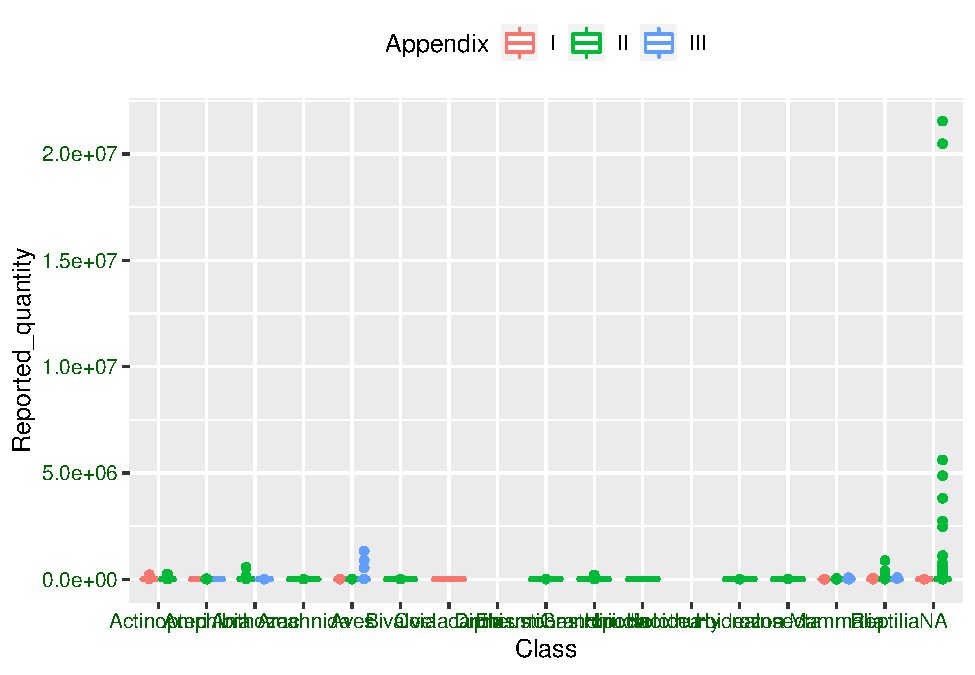
\includegraphics{Wood_ENV872_Project_files/figure-latex/unnamed-chunk-5-1.pdf}

Figure 1. Export Distribution

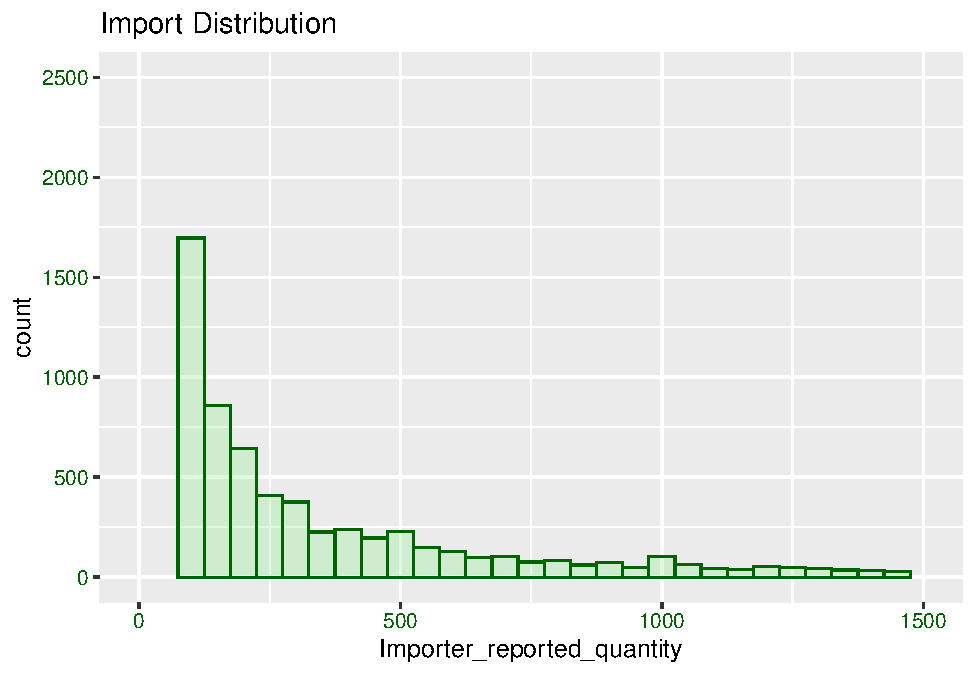
\includegraphics{Wood_ENV872_Project_files/figure-latex/unnamed-chunk-6-1.pdf}

Figure 2. Import Distribution

Next I visualized export quantity and compared to import quantity. I
broke this up by appendix levels which is visualized in Figure 3.
Unfortunately, Appendix I was not easily viewing when combines with
Appendix II and Appendix III so I also visualized that separately in
Figure 4.

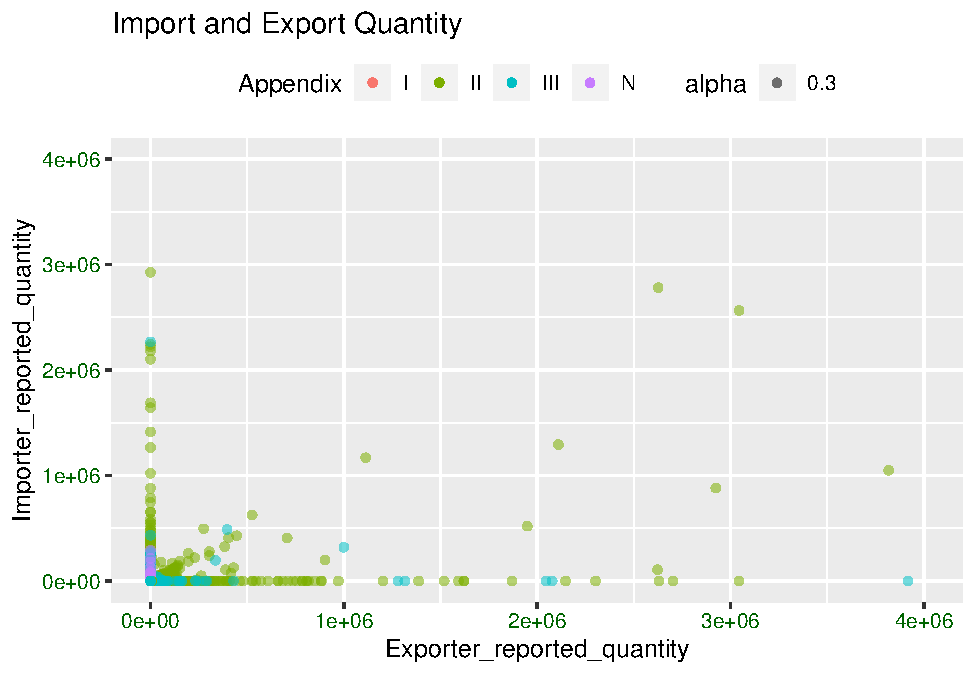
\includegraphics{Wood_ENV872_Project_files/figure-latex/unnamed-chunk-7-1.pdf}

Figure 3. Export and Import Quantity

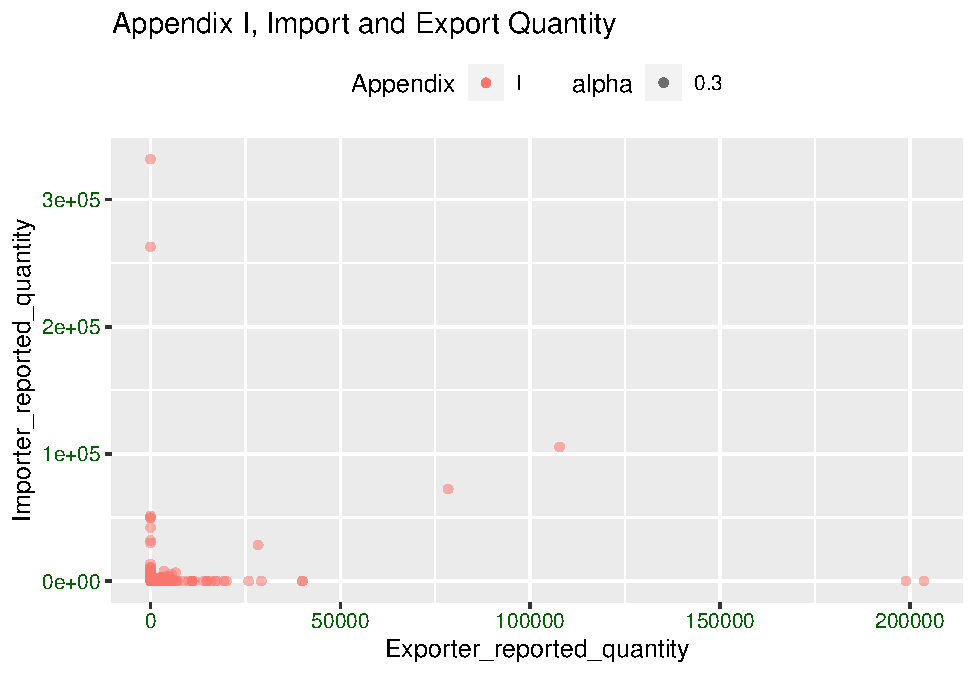
\includegraphics{Wood_ENV872_Project_files/figure-latex/unnamed-chunk-8-1.pdf}

Figure 4. Export and Import Quantity for Appendix I

Next, I visualized the Countries with the most imports and Exports. The
countries with the higher Imports are visualized in Figure 5. For
clarity I also plotted the top ten countries with the most Imports in
Figure 6. I did the same process to visualize exports in Figure 7 and
Figure 8.

Interestingly, we see that the top importers and exporters are
different. The top importer in terms of count is the United stated and
the top exporter in terms of count is the Netherlands. Its important to
note that this could be do to the way they screen their importans and
exports. As there is no accompanied standardization protocol its hard to
say how accurate this is.

\begin{verbatim}
## 59647 codes from your data successfully matched countries in the map
## 1112 codes from your data failed to match with a country code in the map
## 41 codes from the map weren't represented in your data
\end{verbatim}

Figure 5. Importer World Map (In Separate Document)

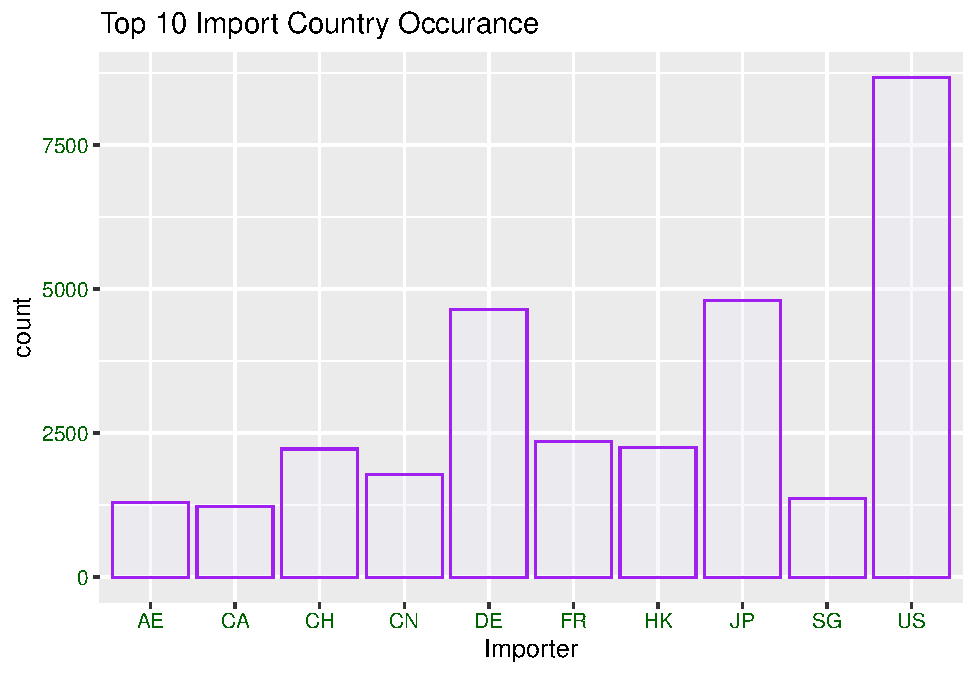
\includegraphics{Wood_ENV872_Project_files/figure-latex/unnamed-chunk-10-1.pdf}

Figure 6. Importer Country Plot Top 10

\begin{verbatim}
## 60130 codes from your data successfully matched countries in the map
## 629 codes from your data failed to match with a country code in the map
## 44 codes from the map weren't represented in your data
\end{verbatim}

Figure 7. Exporter World Map (In Separate Document)

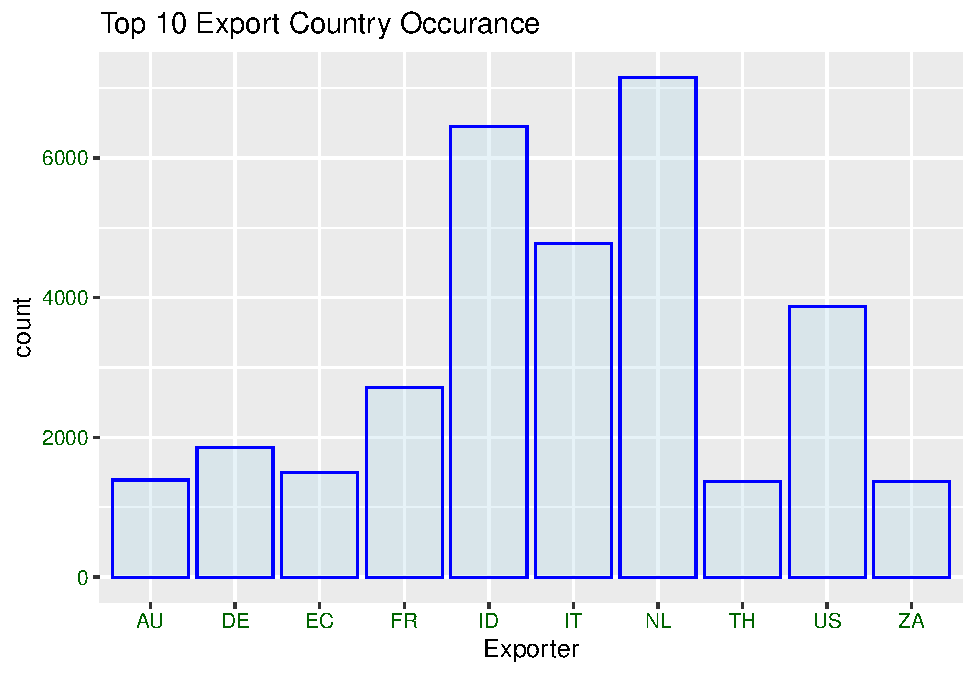
\includegraphics{Wood_ENV872_Project_files/figure-latex/unnamed-chunk-12-1.pdf}

Figure 8. Exporter Country Plot Top 10

Next, I explored the `Class' column. I wanted to know which taxonomic
classes were poached most often. Figure 9 depicts the count for Classes
for the entire dataset. Ass Appendix I contains the subset of species
threatened with extinction by poaching I decided to subset this visually
in Figure 10. From this graph I noted that the top three classes were
Mamilia, Aves, and Reptilia. This was interesting to me as plants are
high risk for poaching because of their transportability. It is then
That I noticed that neither plant Class was represented in this data set
so I decided to explore the NA Class.

Figure 11. shows the breakdown of the Mamilia class by type of good for
Appendix I species. From this information we see that the most common
good type is ivory carvings followed by live animals. In figure 12 we
see the same breakdown for Appendix I Aves. In this figure, we see that
the trade for this class is dominated by live animals. Figure 13 depicts
the breakdown for Reptilia in Appendix I. From this graph we see the
most commonly traded good is small leather products followed by skins.
To explore my hunch that Appendix I plants were hidden in the NAs, I
assigned them a variable and explored the good type breakdown in Figure
14. Here, I saw that the NAs were dominated by live animals followed by
Seeds. From this exploration it is clear that the plant class is
embedded in the Class NAs, but there is not enough information to
conclusively assign them to the plant Classes. More investigation of the
dataframe is needed and this is outside the scope of my project.

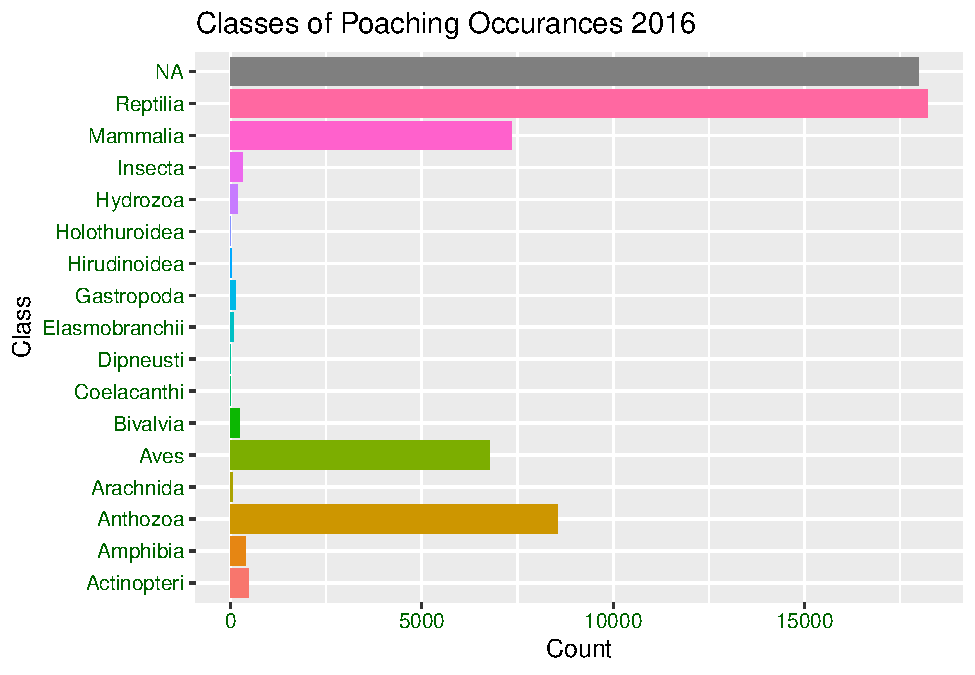
\includegraphics{Wood_ENV872_Project_files/figure-latex/unnamed-chunk-13-1.pdf}

Figure 9. Classes of Poaching Occurrences 2016

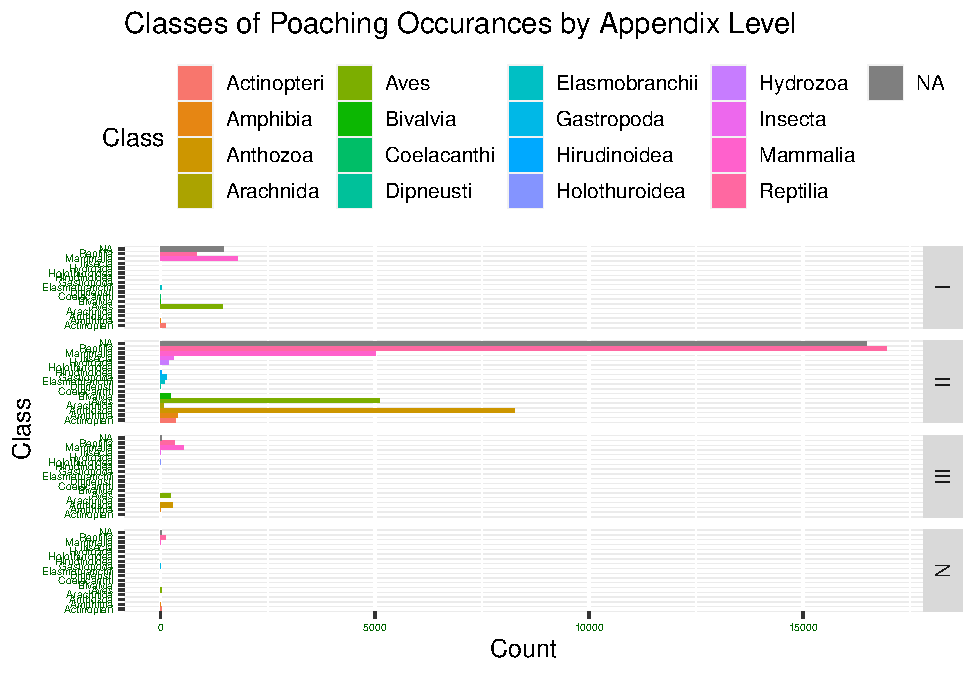
\includegraphics{Wood_ENV872_Project_files/figure-latex/unnamed-chunk-14-1.pdf}

Figure 10. Classes of Poaching Occurrences per Appendix Level

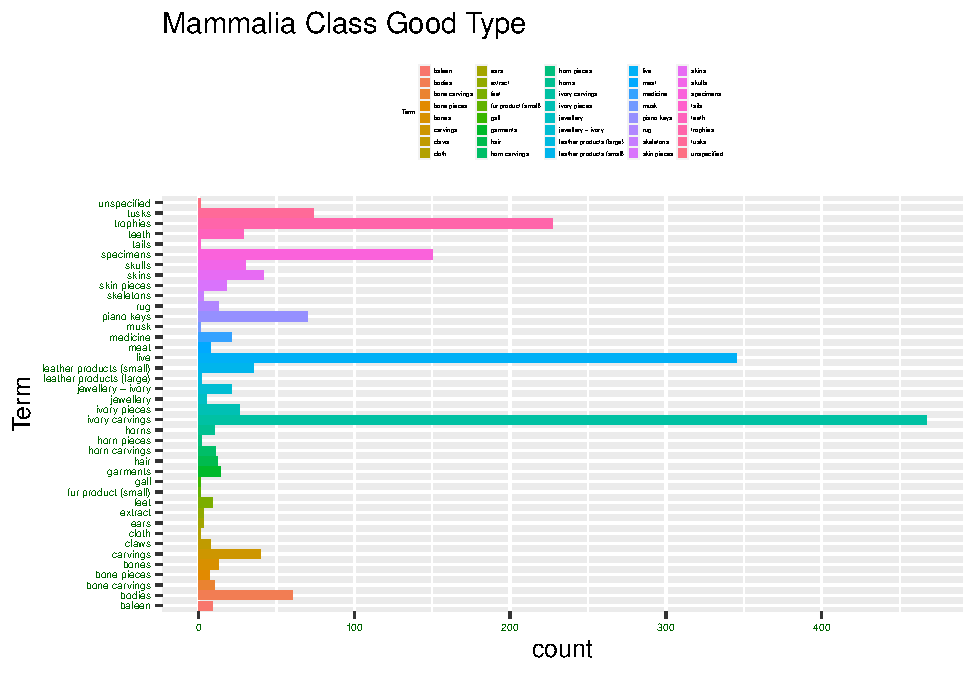
\includegraphics{Wood_ENV872_Project_files/figure-latex/unnamed-chunk-15-1.pdf}

Figure 11. Mammalia Class Good Type

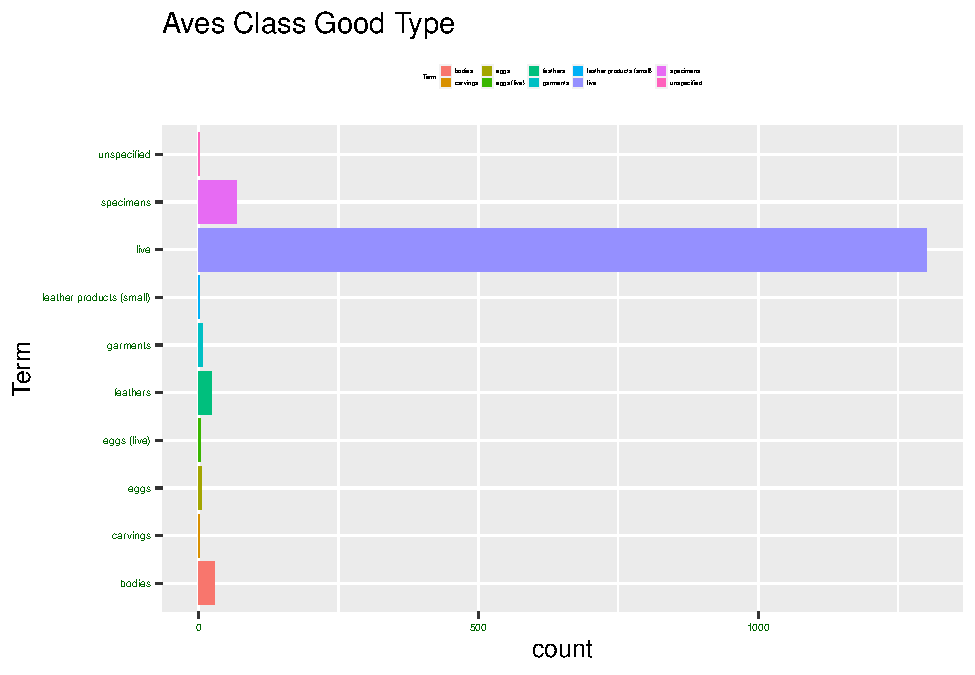
\includegraphics{Wood_ENV872_Project_files/figure-latex/unnamed-chunk-16-1.pdf}

Figure 12. Aves Class Good Type

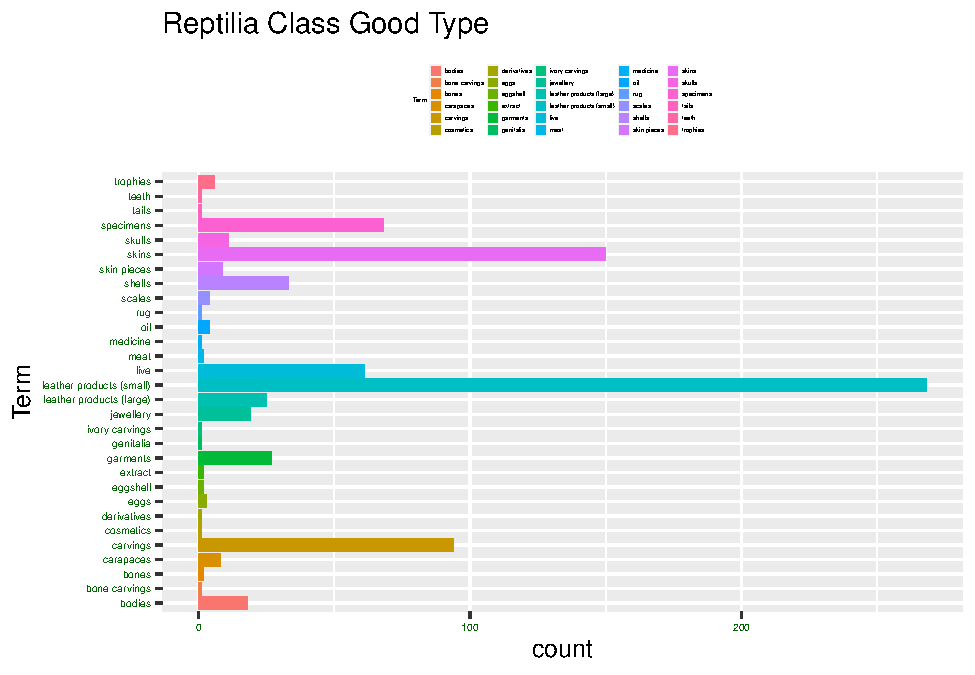
\includegraphics{Wood_ENV872_Project_files/figure-latex/unnamed-chunk-17-1.pdf}

Figure 13. Reptilia Class Good Type

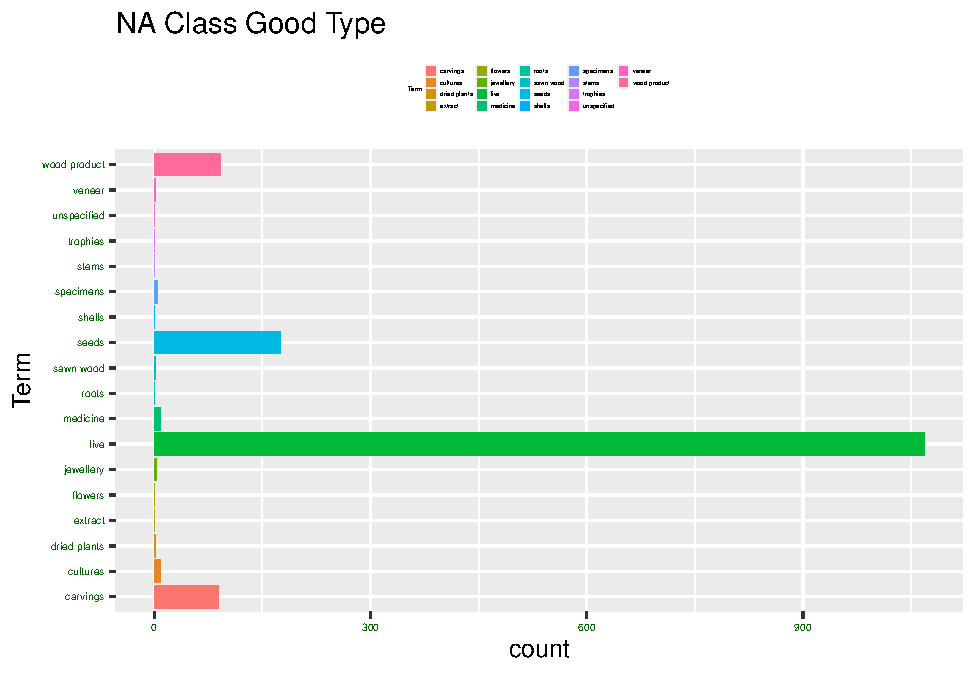
\includegraphics{Wood_ENV872_Project_files/figure-latex/unnamed-chunk-18-1.pdf}

Figure 14. NA Class Good Type

\newpage

\hypertarget{analysis}{%
\section{Analysis}\label{analysis}}

\hypertarget{question-1-is-there-any-correlation-between-class-term-appendix-number-and-total-poaching-amount}{%
\subsection{Question 1: Is there any correlation between class, term,
appendix number and total poaching
amount?}\label{question-1-is-there-any-correlation-between-class-term-appendix-number-and-total-poaching-amount}}

For my main analysis, I wanted to know if the mean of poaching amount
changes according to levels of Class, Term, and Appendix. These last
three variables are categorical. Because of this, I decided to use
two-way ANOVAs to understand the relationship between these variables. I
also wanted to see if the combination of these variables affected the
mean of total poaching amount.

\begin{enumerate}
\def\labelenumi{\arabic{enumi}.}
\tightlist
\item
  For my first model I wanted to know how Poaching Quanitity is
  influenced by Class and Term only within the Appendix I subset.
\end{enumerate}

H: There is no difference in the means of Class in Appendix I H: There
is no difference in means of Term in Appendix I H: There is no
interaction between Class and Term in Appendix I

Null Hypothesis: The alternative hypothesis for cases 1 and 2 is: the
means are not equal.

Null Hypothesis: The alternative hypothesis for case 3 is: there is an
interaction between Class and Term for Appendix I

The summary of our two-way ANOVA (Table. 2) shows us a statistically
significant p-value for Class (DF= 7, P-value = \textless2e-16). This
means that for Class we reject the null hypothesis that the mean across
our groups is different. The p-value for term is also statistically
significant (DF= 52, P-value = \textless0.256). In this case we also
reject the null hypothesis. This model only gives us part of the picture
so I also used a two-way LM.

\begin{verbatim}
##              Df    Sum Sq   Mean Sq F value   Pr(>F)    
## Class         6 4.467e+09 744583316   9.911 1.37e-10 ***
## Term         26 3.259e+09 125332949   1.668   0.0198 *  
## Residuals   853 6.408e+10  75125682                     
## ---
## Signif. codes:  0 '***' 0.001 '**' 0.01 '*' 0.05 '.' 0.1 ' ' 1
## 4768 observations deleted due to missingness
\end{verbatim}

Table 2. Two Way ANOVA Summary

This model gives us a detailed summary of the groups within class which
are significant. The results can be viewed below in Table 3.The results
of this model show high chance of variability (Residual standard error:
4170 on 4132 degrees of freedom). This means that the actual recorded
count can deviate from the true regression line by approximately 4170
occurrences. We also see that our multiple R squared is low (Multiple
R-squared: 0.06678) and therefore our model does not explain the
variance recorded quantity well.

\begin{verbatim}
## 
## Call:
## lm(formula = Reported_quantity ~ Class + Term, data = AppendixI_Facet)
## 
## Residuals:
##    Min     1Q Median     3Q    Max 
## -11288    -54    -40    -11 201942 
## 
## Coefficients:
##                                Estimate Std. Error t value Pr(>|t|)    
## (Intercept)                   1.128e+04  6.391e+03   1.764    0.078 .  
## ClassAmphibia                -1.169e+04  9.028e+03  -1.295    0.196    
## ClassAves                    -1.123e+04  1.542e+03  -7.282 7.46e-13 ***
## ClassCoelacanthi             -1.124e+04  9.390e+03  -1.197    0.232    
## ClassMammalia                -1.127e+04  1.812e+03  -6.220 7.76e-10 ***
## ClassNot_recorded            -1.123e+04  1.521e+03  -7.386 3.59e-13 ***
## ClassReptilia                -1.087e+04  2.602e+03  -4.175 3.28e-05 ***
## Termbodies                   -3.633e+01  7.032e+03  -0.005    0.996    
## Termbones                     2.100e+01  1.062e+04   0.002    0.998    
## Termcarvings                 -2.632e+02  6.612e+03  -0.040    0.968    
## Termcloth                     2.000e+00  1.062e+04   0.000    1.000    
## Termcosmetics                 5.633e+04  1.083e+04   5.204 2.45e-07 ***
## Termeggs                      7.105e+01  7.359e+03   0.010    0.992    
## Termfeathers                 -3.855e+01  1.069e+04  -0.004    0.997    
## Termfeet                     -2.000e+00  8.668e+03   0.000    1.000    
## Termgarments                 -2.610e+02  7.397e+03  -0.035    0.972    
## Termhair                      2.260e+02  1.062e+04   0.021    0.983    
## Termhorn carvings            -2.000e+00  1.062e+04   0.000    1.000    
## Termivory carvings            2.679e+01  6.248e+03   0.004    0.997    
## Termivory pieces              1.570e-11  1.062e+04   0.000    1.000    
## Termleather products (large) -4.078e+02  1.083e+04  -0.038    0.970    
## Termleather products (small) -3.057e+02  6.644e+03  -0.046    0.963    
## Termlive                      1.360e+01  6.230e+03   0.002    0.998    
## Termoil                       1.063e+04  1.083e+04   0.982    0.326    
## Termpiano keys                2.540e+02  7.912e+03   0.032    0.974    
## Termskin pieces               1.765e+03  1.083e+04   0.163    0.871    
## Termskins                     3.111e+02  6.609e+03   0.047    0.962    
## Termskulls                    5.000e+00  8.668e+03   0.001    1.000    
## Termspecimens                 4.168e+02  6.420e+03   0.065    0.948    
## Termteeth                     1.880e+02  8.668e+03   0.022    0.983    
## Termtrophies                  8.776e+00  6.253e+03   0.001    0.999    
## Termtusks                     1.830e+01  6.292e+03   0.003    0.998    
## Termwood product             -1.015e+01  6.776e+03  -0.001    0.999    
## ---
## Signif. codes:  0 '***' 0.001 '**' 0.01 '*' 0.05 '.' 0.1 ' ' 1
## 
## Residual standard error: 8668 on 853 degrees of freedom
##   (4768 observations deleted due to missingness)
## Multiple R-squared:  0.1076, Adjusted R-squared:  0.07412 
## F-statistic: 3.214 on 32 and 853 DF,  p-value: 9.76e-09
\end{verbatim}

Table 3. Two Way LM Summary 2

The Last thing I did for this model was check to see if there was a
relationship between the dependant variables. The results (Table 4) show
a no significant interaction between the variables (P-Value = 0.954).

\begin{verbatim}
##              Df    Sum Sq   Mean Sq F value  Pr(>F)    
## Class         6 4.467e+09 744583316   9.830 1.7e-10 ***
## Term         26 3.259e+09 125332949   1.655  0.0215 *  
## Class:Term    7 1.259e+06    179886   0.002  1.0000    
## Residuals   846 6.408e+10  75745801                    
## ---
## Signif. codes:  0 '***' 0.001 '**' 0.01 '*' 0.05 '.' 0.1 ' ' 1
## 4768 observations deleted due to missingness
\end{verbatim}

Table 4. Two Way ANOVA comparing Class and Term

\begin{Shaded}
\begin{Highlighting}[]
\NormalTok{Poaching}\FloatTok{.2}\NormalTok{way }\OtherTok{\textless{}{-}} \FunctionTok{aov}\NormalTok{(}\AttributeTok{data =}\NormalTok{ AppendixI\_Facet, Reported\_quantity }\SpecialCharTok{\textasciitilde{}}\NormalTok{ Class }\SpecialCharTok{+}\NormalTok{ Term)}

\CommentTok{\# P{-}value is small. Reject our null hypothesis that the mean across our groups}
\CommentTok{\# is different.  Not enough information to tell us which groups are differing}

\NormalTok{Poaching}\FloatTok{.2}\NormalTok{way2lm }\OtherTok{\textless{}{-}} \FunctionTok{lm}\NormalTok{(}\AttributeTok{data =}\NormalTok{ AppendixI\_Facet, Reported\_quantity }\SpecialCharTok{\textasciitilde{}}\NormalTok{ Class }\SpecialCharTok{+}\NormalTok{ Term)}

\CommentTok{\# means are different. Reject null}

\CommentTok{\# TukeyHSD(Poaching.2way)}

\CommentTok{\# check interaction between the variables}

\NormalTok{Poaching}\FloatTok{.2}\NormalTok{way3 }\OtherTok{\textless{}{-}} \FunctionTok{aov}\NormalTok{(}\AttributeTok{data =}\NormalTok{ AppendixI\_Facet, Reported\_quantity }\SpecialCharTok{\textasciitilde{}}\NormalTok{ Class }\SpecialCharTok{*}\NormalTok{ Term)}

\CommentTok{\# Interaction is not significant between variables}
\end{Highlighting}
\end{Shaded}

\begin{enumerate}
\def\labelenumi{\arabic{enumi}.}
\setcounter{enumi}{1}
\tightlist
\item
  For my second model I wanted to know how Poaching Quantity is
  influenced by Class and Appendix for the entire dataframe
\end{enumerate}

H: There is no difference in the means of Class H: There is no
difference in means of Appendix H: There is no interaction between Class
and Appendix

Null Hypothesis: The alternative hypothesis for cases 1 and 2 is: the
means are not equal.

Null Hypothesis: The alternative hypothesis for case 3 is: there is an
interaction between Class and Appendix

The summary of our two-way ANOVA (Table. 5) shows us a statistically
significant p-value for Class (DF= 7, P-value = \textless2e-16). This
means that for Class we reject the null hypothesis that the mean across
our groups is different. The p-value for Appendix is also statistically
significant (DF= 3, P-value = \textless2e-16). In this case we can also
reject the null hypothesis.

\begin{verbatim}
##               Df    Sum Sq   Mean Sq F value Pr(>F)    
## Class         13 1.463e+10 1.125e+09    1.61 0.0745 .  
## Appendix       2 8.712e+10 4.356e+10   62.35 <2e-16 ***
## Residuals   6785 4.740e+12 6.986e+08                   
## ---
## Signif. codes:  0 '***' 0.001 '**' 0.01 '*' 0.05 '.' 0.1 ' ' 1
## 53958 observations deleted due to missingness
\end{verbatim}

Table 5. Model 2 - Two Way ANOVA Summary

This model gives us a detailed summary of the groups within class which
are significant. The results can be viewed below in Table 6.The results
of this model show high chance of variability (Residual standard error:
17690 on 42772 degrees of freedom). This means that the actual recorded
count can deviate from the true regression line by approximately 17690
occurrences. Again, we also see that our multiple R squared is low
(Multiple R-squared: 0.01144) and therefore our model does not explain
all the variance in reported quantity.

\begin{verbatim}
## 
## Call:
## lm(formula = Reported_quantity ~ Class + Appendix, data = CITES2016_Processed)
## 
## Residuals:
##     Min      1Q  Median      3Q     Max 
##  -31209   -2443   -2022    -761 1288663 
## 
## Coefficients:
##                     Estimate Std. Error t value Pr(>|t|)    
## (Intercept)            13105       3274   4.002 6.35e-05 ***
## ClassAmphibia         -13713       4232  -3.240 0.001202 ** 
## ClassAnthozoa         -11972       3380  -3.542 0.000400 ***
## ClassArachnida        -13015      10520  -1.237 0.216079    
## ClassAves             -11703       3350  -3.493 0.000480 ***
## ClassBivalvia         -13445       5845  -2.300 0.021456 *  
## ClassCoelacanthi      -13103      26632  -0.492 0.622749    
## ClassElasmobranchii   -13968      12272  -1.138 0.255043    
## ClassGastropoda         2839       8312   0.342 0.732683    
## ClassHirudinoidea     -11188      18978  -0.590 0.555539    
## ClassHydrozoa         -13835       7049  -1.963 0.049712 *  
## ClassInsecta          -13527       5138  -2.633 0.008492 ** 
## ClassMammalia         -14989       3374  -4.442 9.03e-06 ***
## ClassReptilia         -11495       3322  -3.461 0.000542 ***
## AppendixII               883       1215   0.727 0.467556    
## AppendixIII            29602       2777  10.659  < 2e-16 ***
## ---
## Signif. codes:  0 '***' 0.001 '**' 0.01 '*' 0.05 '.' 0.1 ' ' 1
## 
## Residual standard error: 26430 on 6785 degrees of freedom
##   (53958 observations deleted due to missingness)
## Multiple R-squared:  0.02101,    Adjusted R-squared:  0.01885 
## F-statistic:  9.71 on 15 and 6785 DF,  p-value: < 2.2e-16
\end{verbatim}

Table 6. Model 2 - Two Way LM Summary 2

I decided to check the interaction between Class and Appendix using a
new ANOVA model. In this case, the P-value was statistically significant
(DF= 16, P-value = \textless2e-16). Because of this we accept the Null
hypothesis that there is an interaction between Class and Appendix. This
relationship between Class and Appendix when compared to reported
quantity can be visualized in Figure 15.

\begin{verbatim}
##                  Df    Sum Sq   Mean Sq F value Pr(>F)    
## Class            13 1.463e+10 1.125e+09   1.748 0.0453 *  
## Appendix          2 8.712e+10 4.356e+10  67.690 <2e-16 ***
## Class:Appendix    8 3.787e+11 4.734e+10  73.564 <2e-16 ***
## Residuals      6777 4.361e+12 6.435e+08                   
## ---
## Signif. codes:  0 '***' 0.001 '**' 0.01 '*' 0.05 '.' 0.1 ' ' 1
## 53958 observations deleted due to missingness
\end{verbatim}

Table 7. Model 2 - Two Way ANOVA Comparing Class and Appendix

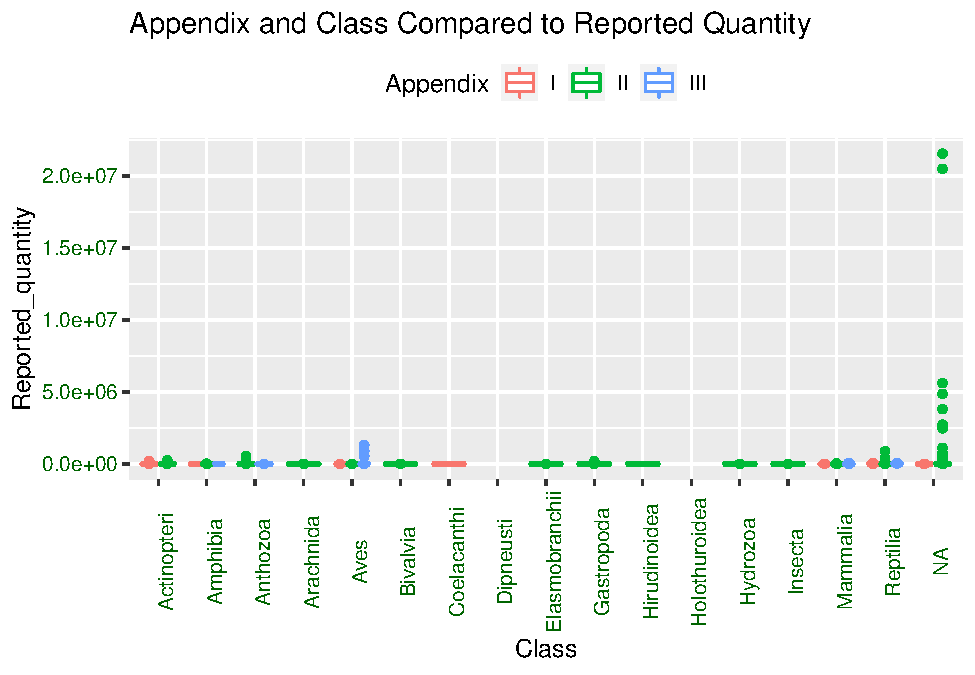
\includegraphics{Wood_ENV872_Project_files/figure-latex/unnamed-chunk-26-1.pdf}
Figure 15. Appendix and Class Compared to Reported Quantity

\begin{Shaded}
\begin{Highlighting}[]
\CommentTok{\# 2. How Does Reported Poaching Quantity vary over Class and Appendix for}
\CommentTok{\# entire data}

\NormalTok{Poaching}\FloatTok{.2}\NormalTok{way.test }\OtherTok{\textless{}{-}} \FunctionTok{aov}\NormalTok{(}\AttributeTok{data =}\NormalTok{ CITES2016\_Processed, Reported\_quantity }\SpecialCharTok{\textasciitilde{}}\NormalTok{ Class }\SpecialCharTok{+}
\NormalTok{    Appendix)}

\CommentTok{\# P{-}value is small. Reject our null hypothesis that the mean across our groups}
\CommentTok{\# is different.  Not enough information to tell us which groups are differing}

\NormalTok{Poaching}\FloatTok{.2}\NormalTok{way2lm.test }\OtherTok{\textless{}{-}} \FunctionTok{lm}\NormalTok{(}\AttributeTok{data =}\NormalTok{ CITES2016\_Processed, Reported\_quantity }\SpecialCharTok{\textasciitilde{}}\NormalTok{ Class }\SpecialCharTok{+}
\NormalTok{    Appendix)}

\CommentTok{\# means are different. Reject null}

\FunctionTok{TukeyHSD}\NormalTok{(Poaching}\FloatTok{.2}\NormalTok{way.test)}
\end{Highlighting}
\end{Shaded}

\begin{verbatim}
##   Tukey multiple comparisons of means
##     95% family-wise confidence level
## 
## Fit: aov(formula = Reported_quantity ~ Class + Appendix, data = CITES2016_Processed)
## 
## $Class
##                                     diff         lwr         upr     p adj
## Amphibia-Actinopteri        -12944.04086  -26971.327   1083.2455 0.1070969
## Anthozoa-Actinopteri        -11235.95598  -22350.741   -121.1712 0.0445431
## Arachnida-Actinopteri       -12527.11301  -47748.305  22694.0794 0.9959387
## Aves-Actinopteri            -10987.64711  -22136.056    160.7616 0.0580844
## Bivalvia-Actinopteri        -12957.77015  -32436.582   6521.0413 0.6061167
## Coelacanthi-Actinopteri     -13497.97015 -102826.805  75830.8651 0.9999998
## Elasmobranchii-Actinopteri  -13480.77015  -54588.024  27626.4833 0.9981976
## Gastropoda-Actinopteri        3326.77985  -24467.802  31121.3612 1.0000000
## Hirudinoidea-Actinopteri    -10699.97015  -74327.749  52927.8086 0.9999991
## Hydrozoa-Actinopteri        -13347.69237  -36887.907  10192.5226 0.8257038
## Insecta-Actinopteri         -13039.12570  -30129.043   4050.7919 0.3669473
## Mammalia-Actinopteri        -12916.68103  -24167.268  -1666.0943 0.0088847
## Reptilia-Actinopteri        -10809.15892  -21752.623    134.3051 0.0568147
## Anthozoa-Amphibia             1708.08488   -7544.368  10960.5378 0.9999973
## Arachnida-Amphibia             416.92785  -34261.622  35095.4779 1.0000000
## Aves-Amphibia                 1956.39374   -7336.424  11249.2114 0.9999869
## Bivalvia-Amphibia              -13.72929  -18493.273  18465.8145 1.0000000
## Coelacanthi-Amphibia          -553.92929  -89670.203  88562.3444 1.0000000
## Elasmobranchii-Amphibia       -536.72929  -41180.003  40106.5448 1.0000000
## Gastropoda-Amphibia          16270.82071  -10832.836  43374.4772 0.7591836
## Hirudinoidea-Amphibia         2244.07071  -61084.941  65573.0820 1.0000000
## Hydrozoa-Amphibia             -403.65152  -23123.932  22316.6294 1.0000000
## Insecta-Amphibia               -95.08485  -16036.689  15846.5188 1.0000000
## Mammalia-Amphibia               27.35982   -9387.795   9442.5149 1.0000000
## Reptilia-Amphibia             2134.88194   -6911.048  11180.8119 0.9999505
## Arachnida-Anthozoa           -1291.15703  -34897.340  32315.0257 1.0000000
## Aves-Anthozoa                  248.30886   -3375.245   3871.8624 1.0000000
## Bivalvia-Anthozoa            -1721.81417  -18100.679  14657.0509 1.0000000
## Coelacanthi-Anthozoa         -2262.01417  -90966.489  86442.4610 1.0000000
## Elasmobranchii-Anthozoa      -2244.81417  -41977.035  37487.4071 1.0000000
## Gastropoda-Anthozoa          14562.73583  -11154.610  40280.0817 0.8270863
## Hirudinoidea-Anthozoa          535.98583  -62212.220  63284.1918 1.0000000
## Hydrozoa-Anthozoa            -2111.73640  -23158.942  18935.4688 1.0000000
## Insecta-Anthozoa             -1803.16973  -15253.389  11647.0499 0.9999999
## Mammalia-Anthozoa            -1680.72506   -5607.406   2245.9562 0.9777372
## Reptilia-Anthozoa              426.79706   -2506.210   3359.8038 0.9999999
## Aves-Arachnida                1539.46589  -32077.852  35156.7842 1.0000000
## Bivalvia-Arachnida            -430.65714  -37649.754  36788.4397 1.0000000
## Coelacanthi-Arachnida         -970.85714  -95762.618  93820.9034 1.0000000
## Elasmobranchii-Arachnida      -953.65714  -52873.243  50965.9284 1.0000000
## Gastropoda-Arachnida         15853.89286  -26316.901  58024.6864 0.9930787
## Hirudinoidea-Arachnida        1827.14286  -69266.678  72920.9633 1.0000000
## Hydrozoa-Arachnida            -820.57937  -40317.146  38675.9875 1.0000000
## Insecta-Arachnida             -512.01270  -36538.425  35514.3993 1.0000000
## Mammalia-Arachnida            -389.56803  -34040.909  33261.7734 1.0000000
## Reptilia-Arachnida            1717.95409  -31831.956  35267.8644 1.0000000
## Bivalvia-Aves                -1970.12304  -18371.824  14431.5780 1.0000000
## Coelacanthi-Aves             -2510.32304  -91219.018  86198.3716 1.0000000
## Elasmobranchii-Aves          -2493.12304  -42234.763  37248.5174 1.0000000
## Gastropoda-Aves              14314.42696  -11417.469  40046.3226 0.8447708
## Hirudinoidea-Aves              287.67696  -62466.494  63041.8476 1.0000000
## Hydrozoa-Aves                -2360.04526  -23425.026  18704.9357 1.0000000
## Insecta-Aves                 -2051.47859  -15529.497  11426.5399 0.9999997
## Mammalia-Aves                -1929.03392   -5949.905   2091.8369 0.9440651
## Reptilia-Aves                  178.48820   -2879.469   3236.4458 1.0000000
## Coelacanthi-Bivalvia          -540.20000  -90675.485  89595.0849 1.0000000
## Elasmobranchii-Bivalvia       -523.00000  -43354.473  42308.4728 1.0000000
## Gastropoda-Bivalvia          16284.55000  -14001.875  46570.9749 0.8748846
## Hirudinoidea-Bivalvia         2257.80000  -62497.300  67012.9002 1.0000000
## Hydrozoa-Bivalvia             -389.92222  -26826.081  26046.2368 1.0000000
## Insecta-Bivalvia               -81.35556  -20980.974  20818.2632 1.0000000
## Mammalia-Bivalvia               41.08912  -16430.234  16512.4121 1.0000000
## Reptilia-Bivalvia             2148.61123  -14114.481  18411.7039 1.0000000
## Elasmobranchii-Coelacanthi      17.20000  -97115.450  97149.8504 1.0000000
## Gastropoda-Coelacanthi       16824.75000  -75465.467 109114.9674 0.9999977
## Hirudinoidea-Coelacanthi      2798.00000 -105799.605 111395.6045 1.0000000
## Hydrozoa-Coelacanthi           150.27778  -90949.048  91249.6038 1.0000000
## Insecta-Coelacanthi            458.84444  -89190.532  90108.2213 1.0000000
## Mammalia-Coelacanthi           581.28912  -88140.305  89302.8828 1.0000000
## Reptilia-Coelacanthi          2688.81123  -85994.360  91371.9826 1.0000000
## Gastropoda-Elasmobranchii    16807.55000  -30390.434  64005.5343 0.9958896
## Hirudinoidea-Elasmobranchii   2780.80000  -71405.487  76967.0871 1.0000000
## Hydrozoa-Elasmobranchii        133.07778  -44691.611  44957.7662 1.0000000
## Insecta-Elasmobranchii         441.64444  -41357.593  42240.8819 1.0000000
## Mammalia-Elasmobranchii        564.08912  -39206.335  40334.5137 1.0000000
## Reptilia-Elasmobranchii       2671.61123  -37013.025  42356.2477 1.0000000
## Hirudinoidea-Gastropoda     -14026.75000  -81749.255  53695.7549 0.9999892
## Hydrozoa-Gastropoda         -16674.47222  -49719.671  16370.7265 0.9188871
## Insecta-Gastropoda          -16365.90556  -45174.042  12442.2308 0.8237102
## Mammalia-Gastropoda         -16243.46088  -42019.790   9532.8682 0.6916709
## Reptilia-Gastropoda         -14135.93877  -39779.707  11507.8293 0.8533184
## Hydrozoa-Hirudinoidea        -2647.72222  -68738.120  63442.6752 1.0000000
## Insecta-Hirudinoidea         -2339.15556  -66416.173  61737.8621 1.0000000
## Mammalia-Hirudinoidea        -2216.71088  -64989.114  60555.6924 1.0000000
## Reptilia-Hirudinoidea         -109.18877  -62827.275  62608.8973 1.0000000
## Insecta-Hydrozoa               308.56667  -24420.196  25037.3290 1.0000000
## Mammalia-Hydrozoa              431.01134  -20688.224  21550.2468 1.0000000
## Reptilia-Hydrozoa             2538.53346  -18418.704  23495.7711 1.0000000
## Mammalia-Insecta               122.44467  -13440.212  13685.1018 1.0000000
## Reptilia-Insecta              2229.96679  -11079.029  15538.9627 0.9999992
## Reptilia-Mammalia             2107.52212   -1304.192   5519.2358 0.7205625
## 
## $Appendix
##             diff       lwr       upr     p adj
## II-I    1229.498 -1405.787  3864.783 0.5179994
## III-I  29383.421 22913.602 35853.240 0.0000000
## III-II 28153.923 22139.310 34168.535 0.0000000
\end{verbatim}

\begin{Shaded}
\begin{Highlighting}[]
\CommentTok{\# check interaction between the variables}

\NormalTok{Poaching}\FloatTok{.2}\NormalTok{way3 }\OtherTok{\textless{}{-}} \FunctionTok{aov}\NormalTok{(}\AttributeTok{data =}\NormalTok{ CITES2016\_Processed, Reported\_quantity }\SpecialCharTok{\textasciitilde{}}\NormalTok{ Class }\SpecialCharTok{*}\NormalTok{ Appendix)}

\CommentTok{\# significant because the pvalue is \textless{}2e{-}16}

\CommentTok{\# TukeyHSD(Poaching.2way3)}

\NormalTok{Poaching.interaction }\OtherTok{\textless{}{-}} \FunctionTok{with}\NormalTok{(CITES2016\_Processed, }\FunctionTok{interaction}\NormalTok{(Class, Appendix))}

\NormalTok{Poaching.anova}\FloatTok{.2}\NormalTok{way5 }\OtherTok{\textless{}{-}} \FunctionTok{aov}\NormalTok{(}\AttributeTok{data =}\NormalTok{ CITES2016\_Processed, Reported\_quantity }\SpecialCharTok{\textasciitilde{}}\NormalTok{ Poaching.interaction)}

\NormalTok{Poaching.groups }\OtherTok{\textless{}{-}} \FunctionTok{HSD.test}\NormalTok{(Poaching.anova}\FloatTok{.2}\NormalTok{way5, }\StringTok{"Poaching.interaction"}\NormalTok{, }\AttributeTok{group =} \ConstantTok{TRUE}\NormalTok{)}

\NormalTok{Poaching.anova.plot }\OtherTok{\textless{}{-}} \FunctionTok{ggplot}\NormalTok{(CITES2016\_Processed, }\FunctionTok{aes}\NormalTok{(}\AttributeTok{y =}\NormalTok{ Reported\_quantity, }\AttributeTok{x =}\NormalTok{ Class,}
    \AttributeTok{color =}\NormalTok{ Appendix)) }\SpecialCharTok{+} \FunctionTok{geom\_boxplot}\NormalTok{() }\SpecialCharTok{+} \FunctionTok{theme}\NormalTok{(}\AttributeTok{axis.text.x =} \FunctionTok{element\_text}\NormalTok{(}\AttributeTok{angle =} \DecValTok{90}\NormalTok{)) }\SpecialCharTok{+}
    \FunctionTok{labs}\NormalTok{(}\AttributeTok{title =} \StringTok{"Appendix and Class compared to Reported Quantity"}\NormalTok{)}
\end{Highlighting}
\end{Shaded}

\newpage

\hypertarget{summary-and-conclusions}{%
\section{Summary and Conclusions}\label{summary-and-conclusions}}

I found that there was a correlation between Class, Term, APpendix and
Reported Quantity. However, I also found that neither of my models was
explaining the variability in our response variable well. More data
analysis is needed to find what else is missing from these models to
better explain this variance.

I was also able to visually compare export and import quantity, as well
as identify and highlight the countries with the highest import and
export amounts. This was accomplished through a bar graphs and a maps
located in an additional document.

Another goal of mine was to explore Appendix I specifically. This
Appendix contains species in which poaching can directly lead to
extinction. I was able to identify the top three classes in the Appendix
and explore the good types that are most commonly traded. I also had
time to explore the case of missing plant classes and identified them
within the NAs.

In conclusion, I have increased the understanding of the CITES 2016
Poaching dataframe. This information can be used to inform policies
surrounding poaching, wildlife trafficking and trade internationally.

\end{document}
